\documentclass[12pt,liststotoc]{report}
\usepackage[T1]{fontenc}
\usepackage[utf8x]{inputenc}
\usepackage{color}
\usepackage{geometry}
\geometry{a4paper, top=25mm, left=25mm, right=25mm, bottom=25mm, headsep=10mm, footskip=12mm} 
\usepackage{amsfonts}
\usepackage{amsmath}
\usepackage[ngerman]{babel}
\usepackage{graphicx}
\usepackage{booktabs}
\usepackage{tabularx}
\usepackage{array}
\usepackage{textcomp}
\usepackage{amssymb}
\usepackage{amstext}
\usepackage{subfigure}
\usepackage{amsfonts}
\usepackage{mathrsfs}
\usepackage{csquotes}
\usepackage{multirow}
\usepackage{color}
\usepackage{bigstrut}
\usepackage[version=4]{mhchem}
\usepackage{textcomp} 
\usepackage{nicefrac}
\usepackage{caption}
\usepackage{lmodern}
\usepackage{pdflscape}
\usepackage{pdfpages}
\usepackage{here} 
\newcommand{\rtab}{\raggedleft\arraybackslash}

\usepackage{hyperref}
\usepackage{fancyref}
\usepackage{todonotes}
\usepackage{bigints}
\usepackage{amsmath}
\usepackage{amssymb}
\usepackage{amstext}
\usepackage{amsfonts}
\usepackage{mathrsfs}
\usepackage[version-1-compatibility]{siunitx}

%\usepackage[backend=biber,style=alphabetic,sorting=ynt]{biblatex}
%\addbibresource{Quelle_CRT_2.bib} 
 



\usepackage{ngerman}
\setlength{\parindent}{0em}	
\setlength{\parskip}{1.5ex plus0.5ex minus0.5ex}

\usepackage{chemformula}

\captionsetup[table]{skip=5pt}


\begin{document}
\setcounter{secnumdepth}{5}
\setcounter{tocdepth}{5}

\begin{titlepage}
	\centering
	
\includegraphics[width=0.5\textwidth]{Graphics/TU_Graz.pdf}\par\vspace{1cm}
	
	{\scshape\LARGE Reaktionstechnik II LU  \par}
	\vspace{1cm}
	{\scshape\Large LU 667.212\par}
	{\scshape \large SS 2018\par}
	\vspace{0.5cm}
	{\huge\bfseries Verweilzeitverteilung\par}
	\vspace{0.5cm}

	{\LARGE \itshape Ashok Andermann\par}
	{\large 11729115\par}\vspace{0.5cm}
	%\vspace{0,2cm}	
	
	{\LARGE \itshape Kilian Fleisch\par}
	{\large 11744809\par}\vspace{0.5cm}
	%\vspace{0,2cm}
	
		
	{\LARGE \itshape Jakob Geistlinger\par}
	{\large 01131349\par}\vspace{0.5cm}
	%\vspace{0,2cm}
	
	{\LARGE \itshape Felix Lechleitner\par}
	{\large 01316701\par}\vspace{0.5cm}
	%\vspace{0,2cm}

	{\LARGE \itshape Tobias Maier\par}
	{\large 01330853\par}\vspace{0.5cm}
	%\vspace{0,2cm}
	\vfill

% Bottom of the page
	{\large \today\par}
\end{titlepage}


\pagenumbering{Roman}
\tableofcontents
\newpage
\pagenumbering{arabic}
\chapter{Einleitung \& Aufgabenstellung}

\par Rohrreaktoren werden in der Industrie häufig eingesetzt, z.B. für die Synthese von Polyamid bzw. allgemein für Polymerisationsreaktionen. \cite{fogler1999elements,Chemgapedia}
Um große Volumina erreichen zu können werden Rohrbündelreaktoren aus mehreren einzelnen Rohrreaktoren verwendet. Im Rahmen dieses Experiments werden die realen Verweilzeitverteilungen von zwei Kunststoffrohrreaktoren aus REHAU-rauclair-e $\copyright$ mit und ohne Füllkörpern verglichen, wobei die Füllkörper Glaskugeln mit Durchmesser $\approx$ 1\,mm sind. 
\\
\\
Basierend darauf sollten theoretische Vergleiche mit verschiedenen idealen Reaktoren angestellt und die Effekte auf eine hypothetisch darin ablaufende Reaktion diskutiert werden. Dazu wird einerseits die Puls- und andererseits die Stufenfunktion analysiert, wobei als Tracer eine NaCl-Lösung verwendet wird. In weiterer Folge kann die Altersverteilung und die kumulative Verteilung ermittelt werden um daraus die mittlere Verweilzeit, Varianz und verschiedene Vergleiche mit dem Dispersions- und Kaskadenmodell anzustellen. Des Weiteren kann der Einfluss der Verweilzeitverteilung auf eine hypothetisch im Reaktor ablaufende Reaktion diskutiert werden.


%\par Ziel dieser Laborübung war die Bestimmung der Verweilzeitverteilung zweier Rohrreaktoren.
%Basierend darauf sollten theoretische Vergleiche mit verschiedenen idealen Reaktoren angestellt und die Effekte auf eine hypothetisch darin ablaufende Reaktion diskutiert werden.

%\par Die Verweilzeitverteilung wurde jeweils durch eine Stoßfunktion sowie eine Sprungfunktion experimentell ermittelt. Daraus wurde die mittlere Verweilzeit und die Varianz berechnet, und die Daten mit idealen Reaktoren Verglichen. 



\chapter{Versuchsaufbau}


Als Fluid ohne Tracer ($H_2O$) wird nicht reines deionisiertes verwendet aber mit Leitungswasser vermischt. Deionisiertes Wasser wird mit Leitungswasser vermischt damit immer eine Grundleitfähigkeit vorhanden ist, reines deionisiertes Wasser hätte ebenfalls eine Leitfähigkeit die nicht bei 0 liegt sondern ca. 50\,$\mu$S/cm \cite{Leitfahigkeit_Wasser}. Wäre der Wert der Leitfähigkeit $\kappa$ gleich 0 ergeben sich mit der gewählten Berechnungsmethode für $E(t)$ Werte gegen $\infty$.

%\begin{figure}[H]
%\centering
%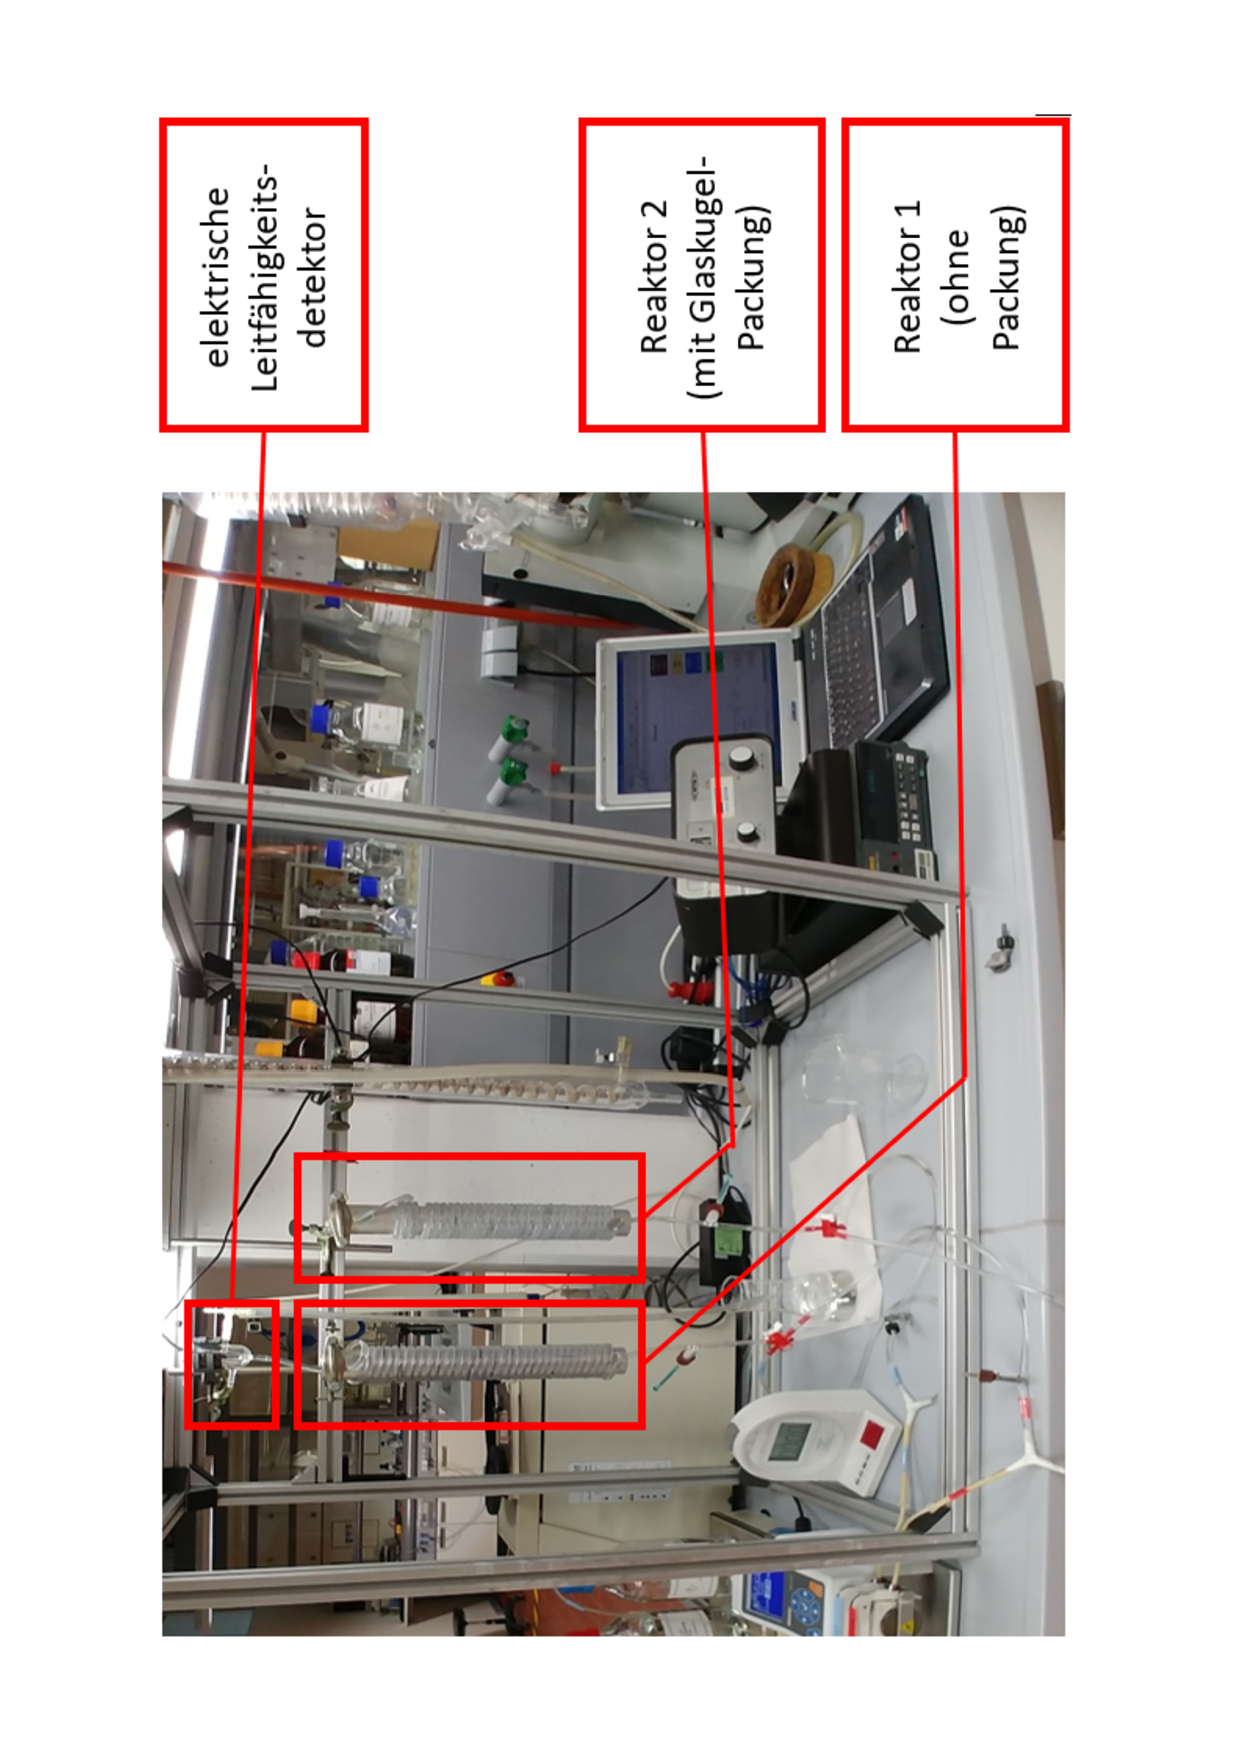
\includegraphics[angle=270,width=0.8\textwidth]{Graphics/Versuchsaufbau.pdf} 
%\caption{Versuchsaufbau [1] (Skript Labor)}
%\label{Versuchsaufbau}
%\end{figure}
%\noindent

Der Versuchsaufbau besteht aus zwei verschiedenen „plug-flow-reactors“ (PFRs), einer Schlauchquetsch-Pumpe, zwei Lagertanks, einer mit H$_2$O und einer mit in Wasser gelösten NaCl (Marker / Tracer), einem Chronometer und einer Leitfähigkeitszelle.
\\
\\
Die beiden Reaktoren sind als 5\,m lange Kunststoffrohre mit einem inneren Durchmesser von 5\,mm ausgeführt, die auf einem Metallrohr aufgewickelt sind. Ein Reaktor ist mit Glaskugeln gefüllt, während der andere keine Packung aufweist. Der Aufbau des Experiments ist in Abbildung \ref{Versuchsaufbau} zu sehen. Abbildung \ref{Prozessfliessbild} zeigt das Prozessfließbild des Versuchs. Am Ende der beiden Reaktoren befindet sich ein Leitfähigkeitsdetektor, der die Konzentration an Tracer bestimmt.

%\todo{Abmaße Reaktor}

\begin{figure}[H]
\centering
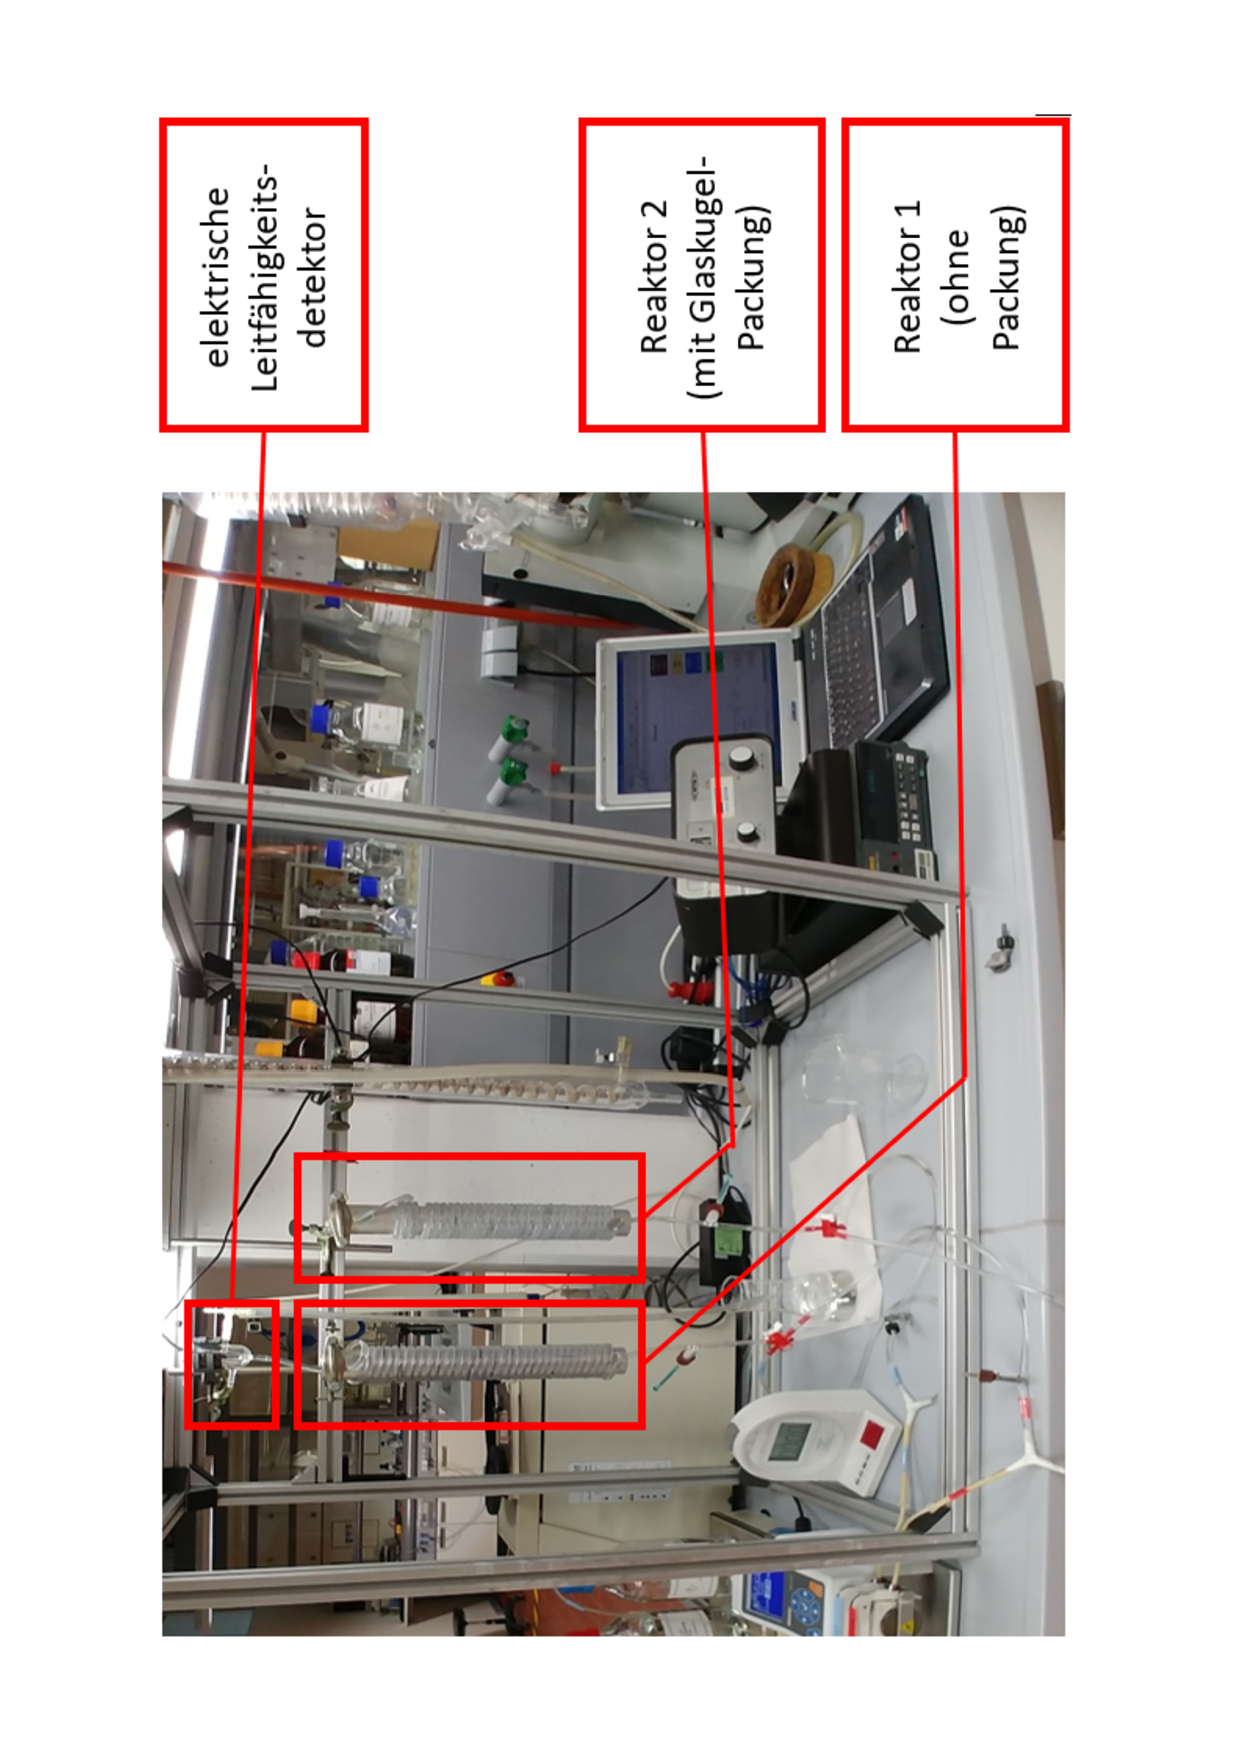
\includegraphics[angle=270,width=1\textwidth]{Graphics/Versuchsaufbau.pdf} 
\caption[Versuchsaufbau des Experiments zur Bestimmung der Verweilzeitverteilung zweier PFRs mit NaCl als Tracer]{Versuchsaufbau des Experiments zur Bestimmung der Verweilzeitverteilung zweier PFRs mit NaCl als Tracer \cite{Skript_2018}}
\label{Versuchsaufbau}
\end{figure}
\noindent

\begin{figure}[H]
\centering
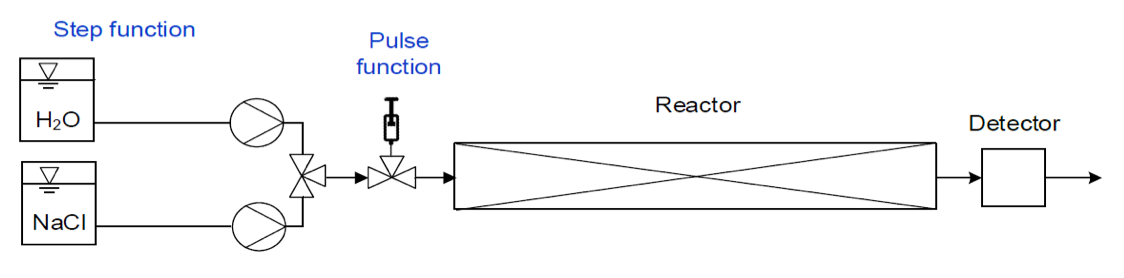
\includegraphics[width=0.8\textwidth]{Graphics/Prozessfliessbild.png} 
\caption[Prozessfließbild des Versuchs]{Prozessfließbild des Versuchs \cite{Skript_2018}}
\label{Prozessfliessbild}
\end{figure}
\noindent






\chapter{Durchführung}

%Zu Beginn wird eine Kalibrationskurve der Schlauchquetschpumpe erstellt. Dazu wird die Zeit gemessen, welche benötigt wird um eine bestimmte Masse zu fördern, in diesem Falle 5\,g. 


Vor Beginn der Versuche muss eine Kalibration der Schlauchquetsch-Pumpe durchgeführt werden, um den genauen Durchfluss der Pumpe zu bestimmen. Dabei wird das Gewicht des Fluiddurchsatzes nach einer gewissen Zeit gemessen. Die Menge wird durch die Zeit geteilt, um einen Wert für die Durchflussrate zu ermitteln. In Tabelle \ref{tab:Pumpenkalibration} sind die Ergebnisse der Pumpenkalibration dargestellt. Über die Dichte wird der gemessene Massenstrom in den Volumenstrom übergeführt, wobei zur Ermittlung der Pumpenkennlinie eine Dichte von reinem Wasser mit $\rho_{H_2O}$= 1000\,$\text{kg}\cdot{\text{m}^{-3}}$ herangezogen wird.

\begin{align}
\dot{m} =&\; \frac{m}{\Delta t} \\
\dot{V} =&\; \dot{m} \cdot \rho
\end{align} 

Nach der Kalibration der Pumpe können die Versuche durchgeführt werden. Zwei verschiedene Injektionsarten (Pulsunktion und Stufenfunktion) werden verwendet. Für die Versuche werden drei unterschiedliche Volumenströme im Reaktor gewählt. Tabelle \ref{tab:Volumenströme} zeigt die Umdrehungszahlen der Pumpe für die verschiedenen Durchsätze, die für beide Reaktoren gleich sind.
\\
\\
In den Pulsfunktionsexperimenten wird der Reaktor mit deionisiertem Wasser betrieben und der Tracer wird über eine kurze Zeit (quasi instantan) über eine Spritze injiziert. Bei der Injektion ist unbedingt darauf zu achten, dass der Auslass der Spritze in Strömungsrichtung zeigt, um das Strömungsverhalten möglichst wenig zu beeinflussen. Abbildung \ref{Injektionsvorrichtung} zeigt die Strömungsrichtung und die Injektionsvorrichtung für die Pulsfunktion. Das Experiment gilt als abgeschlossen, sobald die Konzentration des Tracers am Ausgang des Reaktors gegen Null geht bzw. die „Startkonzentration“ wieder erreicht wird.

\begin{figure}[H]
\centering
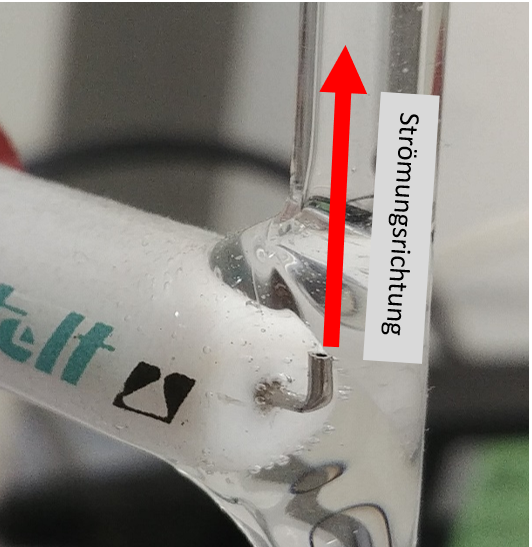
\includegraphics[width=0.5\textwidth]{Graphics/Injektionsvorrichtung.PNG}
\caption{Injektionsvorrichtung für die Pulsfunktion}
\label{Injektionsvorrichtung}
\end{figure}
\noindent
In den Stufenfunktionsversuchen wird der Reaktor zunächst mit deionisiertem Wasser betrieben und am Startpunkt wird das Dreiwegeventil geschaltet, um das Wasser mit dem Tracer nun kontinuierlich durch den Reaktor zu transportieren. Das Experiment gilt als abgeschlossen, sobald die Konzentration des Tracers am Ausgang des Reaktors ca. konstant ist. Zur Bestimmung des Durchflusses aus der Pumpenkalibrierung wird die Masse (5\,g) durch die Zeit in min dividiert, in weiterer Folge wird die Dichte zur Bestimmung des Volumenstroms in $\text{ml}\cdot\text{min}^{-1}$ herangezogen. 

\begin{table}[H]
\centering
\caption[Pumpenkalibration]{Die Zeit um 5\,g an deionisiertem Wasser zu transportieren wird bei verschiedenen Umdrehungszahlen der Pumpe gemessen, um die Durchflussrate zu bestimmen}
\begin{tabular}{ccc}
\toprule 
Drehzahl in $\frac{1}{\text{min}}$ & Zeit in s & Durchfluss in $\frac{\text{g}}{\text{min}}$\\
\midrule
10 & 119 & 2,52\\
20 & 78 & 3,85 \\
30 & 56 & 5,36 \\
40 & 30 & 10,00 \\
50 & 24 & 12,50 \\
\bottomrule
\end{tabular}
\label{tab:Pumpenkalibration}
\end{table}
\noindent

\begin{table}[H]
\centering
\caption{Umdrehungen pro Minute der Pumpe für die Volumenströme der Versuche}
\begin{tabular}{cc}
\toprule 
Drehzahl in $\frac{1}{\text{min}}$ & Volumenstrom in $\frac{\text{ml}}{\text{min}}$\\
\midrule
27 & 7 \\
38 & 10 \\
49 & 13 \\
\bottomrule
\end{tabular}
\label{tab:Volumenströme}
\end{table}
\noindent



\chapter{Ergebnisse $\&$ Interpretation}

\section{Bestimmung der Verweilzeitverteilung für Stufen- und Pulsfunktion}


   
 %  \missingfigure{Versuche deklarieren, Versuch 1-3 im Reaktor 1 \& Versuch 1-3 im Reaktor 2, dass referenziert werden kann}

Aus den detektierten Werten, welche die Leitfähigkeit der verwendeten NaCl-Lösung darstellen, kann mittels dem abgeänderten Kohlrauschgesetz \cite{Leitfahigkeit_Wasser} in die Konzentration umgerechnet werden. In den weiterführenden Berechnungen wird die Konzentration verwendet. Die Berechnung der Konzentration ist beispielhaft für den ersten Versuch (siehe Tabelle \ref{tab:Versuchsnummerierung}) für NaCl ($\kappa = 0,1813\,\frac{\text{S}}{\text{cm}}$; t = 122 s) durchgeführt:

\setlength\jot{0,5cm}
\begin{align}
    \Lambda_0(\text{NaCl})=&\;n\cdot\Lambda^+_0(\text{Na}^+) + m\cdot\Lambda^-_0(\text{Cl}^-)\\
    &\text{mit } n\;\text{Na-}\text{Atome } \text{und } m\; \text{Cl-}\text{Atome}\notag\\
    \Lambda_0(\text{NaCl})=&\;1\cdot50,1\,\frac{\text{S}\cdot\text{cm}^2}{\mole} + 1\cdot76,8\,\frac{\text{S}\cdot\text{cm}^2}{\mole} = 126,9\,\frac{\text{S}\cdot\text{cm}^2}{\mole}\notag\\
    c (t_i) = &\;\frac{\kappa(t_i)}{\Lambda_0(\text{NaCl})}\\
    c (122\,\s) = &\; \frac{0,1813\,\frac{\text{S}}{\text{cm}}}{126,9\,\frac{\text{S}\cdot\text{cm}^2}{\mole}\cdot1000} \approx 0,0014\,\frac{\mole}{\litre}\notag
\end{align}



\begin{figure}[H]
\centering
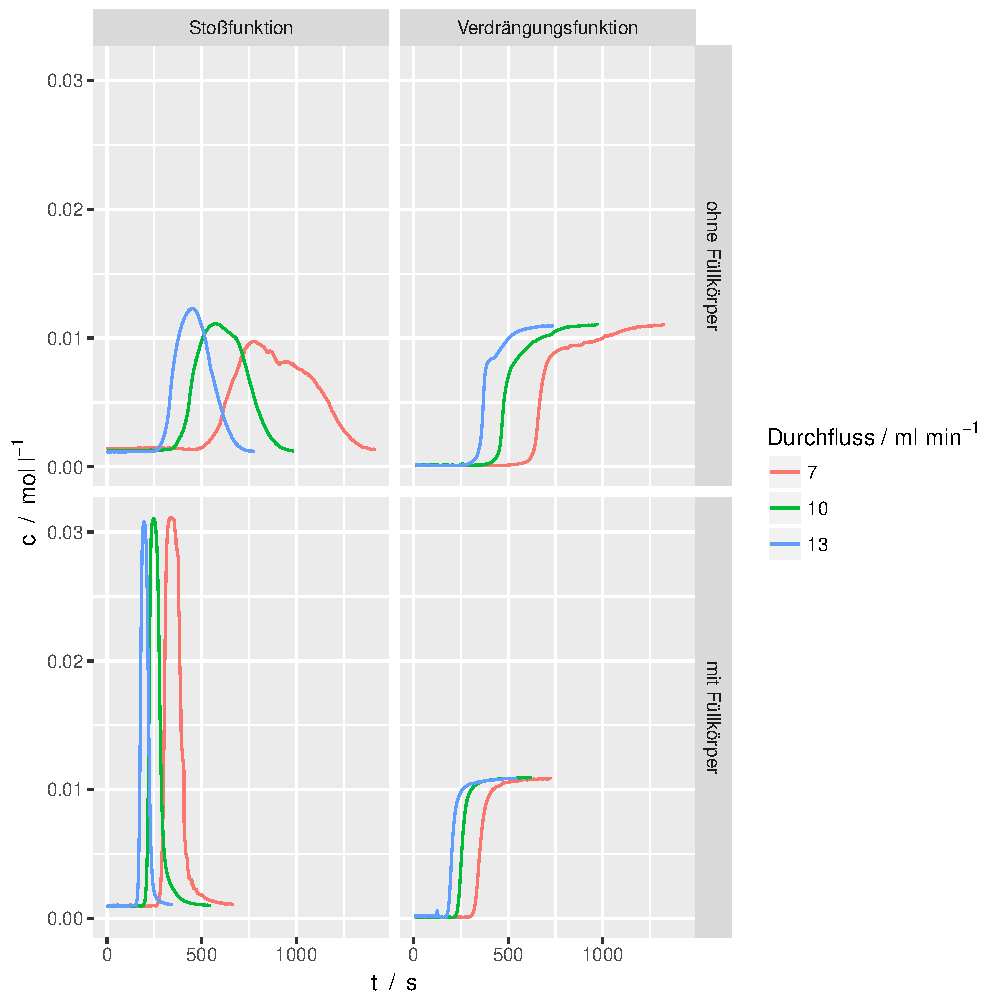
\includegraphics[width=1\textwidth]{Graphics/ct.pdf}
\caption[Konzentrationsverläufe]{Konzentrationsverläufe der einzelnen Versuche}
\label{konzentrationsverlauf}
\end{figure}
\noindent
In Abbildung \ref{konzentrationsverlauf} ist der Konzentrationsverlauf der einzelnen Versuche dargestellt, links für die Pulsfunktion und rechts für die Stufenfunktion. Im weiteren Verlauf der Darstellung der Ergebnisse werden die Versuche nummeriert um eine einfachere Zuweisung zu ermöglich. Diese Nummerierung ist in Tabelle \ref{tab:Versuchsnummerierung} dargelegt. Die Stufenfunktion beim Reaktor ohne Füllkörper zeigt einen breiteren Verlauf, was in weiteren Berechnungen auch am höheren Wert der Varianz (dem Quadrat der Standardabweichung) erkennbar ist. Auch die Stufenfunktion zeichnet sich durch einen nicht idealen Verlauf aus. Das bedeutet, dass der Reaktor mit Füllkörpern sich realer verhält als der ohne. Ebenfalls ist zu sehen, dass der Tracer bei dem Reaktor mit Füllkörper schneller durch den Reaktor gelangt, als beim Reaktor  ohne Füllkörper. Dies ist auf das im Vergleich kleinere Volumen im Reaktor mit Füllkörpern zurückzuführen. Dies ist rechnerisch wie folgt zu verstehen, wobei die Indizes OFK und MFK  für \underline{o}hne \underline{F}üll\underline{k}örper und \underline{m}it \underline{F}üll\underline{k}örper stehen:

%\todo{Berechnung der Volumen der Reaktoren}

\begin{align}
    V_{OFK}=&\;\frac{d^2\cdot\pi}{4}\cdot L =          \notag \frac{0,005^2\,\m^2\cdot\pi}{4}\cdot5\,\m = 98,18\,\text{ml} \\ \notag
    V_{MFK}=&\; \dot{V} \cdot \bar{t} = 41,15\,\text{ml} \notag
\end{align}


Das Volumen des Reaktors mit Füllkörpern wird mit der mittleren Verweilzeit, welche als hydraulische Verweilzeit $\tau$ angenommen wird, für den Versuch bei $\dot{V}$=7\,$\text{ml}\cdot\text{s}^{-1}$ berechnet. Somit kann in weiterer Folge die Menge an Glaskugeln im Reaktor bei bekanntem Durchmesser der Kugeln von ca. 1\,mm und der Differenz der Volumina der beiden Reaktoren abgeschätzt werden (Anzahl Kugeln $\approx$ 31587). \\
Des Weiteren zeigt sich sehr markant beim Durchfluss von $7\,\mole\cdot\litre^{-1}$ bei ca. 900\,s eine Unebenheit in der Kurve. Diese Unebenheit ist auf Luftblasen zurückzuführen, welche während dem Versuch aufgetreten sind.

\begin{table}[H]
\centering
\caption{Versuchsnummerierung mit Versuchsparametern}
\begin{tabular}{c|c|c|cc}
\toprule 
Versuchsnummer $\#$ & Reaktor & Volumenstrom in $\frac{\text{ml}}{\text{min}}$ & Experiment \\
\midrule
1 & ohne Füllk.& 7 & Puls \\
2 & ohne Füllk. & 10 & Puls \\
3 & ohne Füllk. & 13 & Puls \\
4 & mit Füllk. & 7 & Puls \\
5 & mit Füllk. & 10 & Puls \\
6 & mit Füllk. & 13 & Puls \\
7 & ohne Füllk. & 7 & Stufen \\
8 & ohne Füllk. & 10 & Stufen \\
9 & ohne Füllk. & 13 & Stufen \\
10 & mit Füllk. & 7 & Stufen\\
11 & mit Füllk. & 10 & Stufen \\
12 & mit Füllk. & 13 & Stufen\\
\bottomrule
\end{tabular}
\label{tab:Versuchsnummerierung}
\end{table}
\noindent
\newpage 

\section{Pulsfunktion}

Im Rahmen der Ermittlung der Verweilzeitverteilung mittels der Pulsfunktion werden ca. 0,4\,ml einer NaCl-Lösung mit einer Spritze in den Rohrreaktor an einer Stelle zwischen der Schlauchquetschpumpe, welche weiterhin das Gemisch aus demineralisiertem H$_2$O und Leitungswasser fördert, und dem aufgewickelten Rohr, injiziert. Damit sollte im Idealfall am Ausgang des Reaktors an der Messstelle ein starkes Signal in einem engen Zeitintervall gemessen werden. Im realen Fall ist das Signal aber über einen längeren Zeitraum detektierbar und muss daher über die gemessene Leitfähigkeit bzw. die daraus resultierende Konzentration beschrieben werden. Die dazu notwendigen Gleichungen sind aus Quelle \cite{Skript_2018,Chem_Reaktion_2018} entnommen.
 
\subsection{Verweilzeitdichtefunktion E(t) aus Pulsfunktion}

Das Ergebnis der Pulsfunktion ist ein Peak im Konzentrations-Zeit-Diagramm. Dieser Peak wird in die sogenannte Verweilzeitdichteverteilung umgerechnet. Das Integral dieser Kurve, sprich die Fläche unter der Kurve, entspricht dem Wert 1. Bei Diskretisierung der Zeitschritte lässt sich die Summe numerisch generieren. Die Verweilzeitdichteverteilung ist wie folgt charakterisiert:

\begin{align}
E(t) =&\;\frac{c_{i}}{\int_{0}^{\infty} c_{i}\cdot \text{d}t_i}\,\approx\,\frac{c_i}{\sum c_i \cdot \Delta t_i}\\
\textit{mit }\sum c_i \cdot \Delta t_i =&\; c_1\cdot\Delta t_1 + c_2\cdot\Delta t_2 +\;...\;+c_n \cdot \Delta t_n \\
\sum c_i \cdot \Delta t_i =&\; 0,0014\,\frac{\mole}{\litre} \cdot 3\,\s + 0,0015\,\frac{\mole}{\litre}\cdot 3\,\s +\;...\notag\\
&...\;+0,0013\,\frac{\mole}{\litre} \cdot 3\,\s \approx 5,91\,\frac{\mole\cdot\s}{\litre}\notag\\\notag
\end{align}

Für die beispielhafte Konzentration von $0,009\,\mole\cdot\litre^{-1}$ bei Sekunde 864 ($\Delta t = 3\,\s$) ergibt sich folgender Wert für die Funktion $E(t)$:

\begin{equation*}
E(864\,\s) = \frac{0,009\,\frac{\mole}{\litre}}{5,91\,\frac{\,\mole\cdot\s}{\litre}} \approx0,0015\,\frac{1}{\s}
\end{equation*}

Mit Hilfe der Progammiersprache \textit{R} werden die im Laufe des Versuchs generierten Werte aus \textit{Excel} zu den jeweiligen Zeitpunkten eingelesen und es werden nach obigem Rechenschema die dazugehörigen Werte für die Verweilzeitdichtefunktion kalkuliert. Die Start- und End-Zeitpunkte für die jeweiligen Versuche werden händisch laut den dokumentierten Werten eingelesen. Die weiteren Berechnungen  werden ebenfalls mit dieser Datenauswertungsmethode durchgeführt.

\begin{figure}[H]
\centering
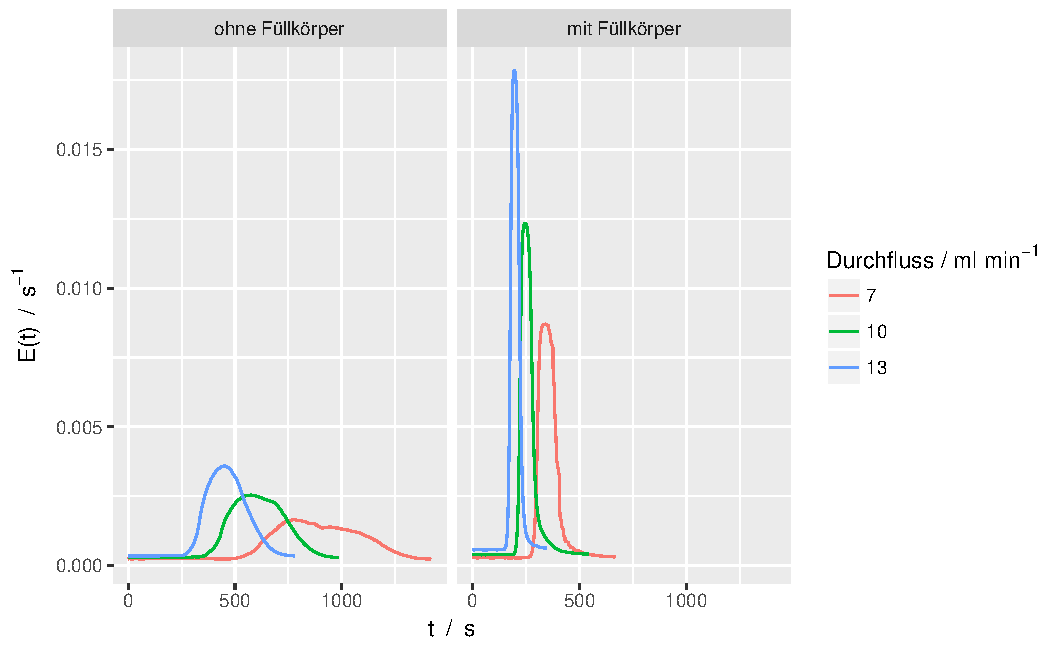
\includegraphics[width=1\textwidth]{Graphics/E_stoss.pdf}
\caption[Verweilzeitdichte Pulsmarkierungen]{Verweilzeitdichten aus der Pulsmarkierung}
\label{dichte_stoss}
\end{figure}
\noindent





\subsection{Verweilzeitsummenfunktion F(t)}

Aus der Verweilzeitdichtefunktion kann durch das Integral in Abhängigkeit der Zeit die Verweilzeitsummenfunktion generiert werden. Die Funktion F(t) ist eine prozentuelle Angabe und hat ihr Maximum demnach bei 1, ist einheitenlos und beschreibt die Zeitspanne in welcher der gesamte Tracer den Ausgang des Reaktors passiert hat bzw. das Maximum, sprich die Konzentration der zugeführten Lösung, gemessen wird. Bei numerischer Lösung des Integrals wird folgende Gleichung für die Berechnung der Summenfunktion angewandt:

\begin{align}
F(t) =&\; \int_{0}^{t} E(t_i) \cdot \text{d} t_i \approx \sum E(t_i) \cdot \Delta t_i\\
F(t_n) =&\;E(t_1) \cdot \Delta t_1 + E(t_2) \cdot \Delta t_2+\;...\;+E(t_n) \cdot \Delta t_n\\\notag
\end{align}

Für 553\,s ergibt sich folgender Wert:

\begin{equation*}
F(553\,\s) =0,0002\,\frac{1}{\s}\cdot 3\,\s + 0,0002\,\frac{1}{\s}\cdot3\,\s+\;...\;+ 0,0004\,\frac{1}{\s} \cdot 3\,\s \approx 0,1137
\end{equation*} 

\begin{figure}[H]
\centering
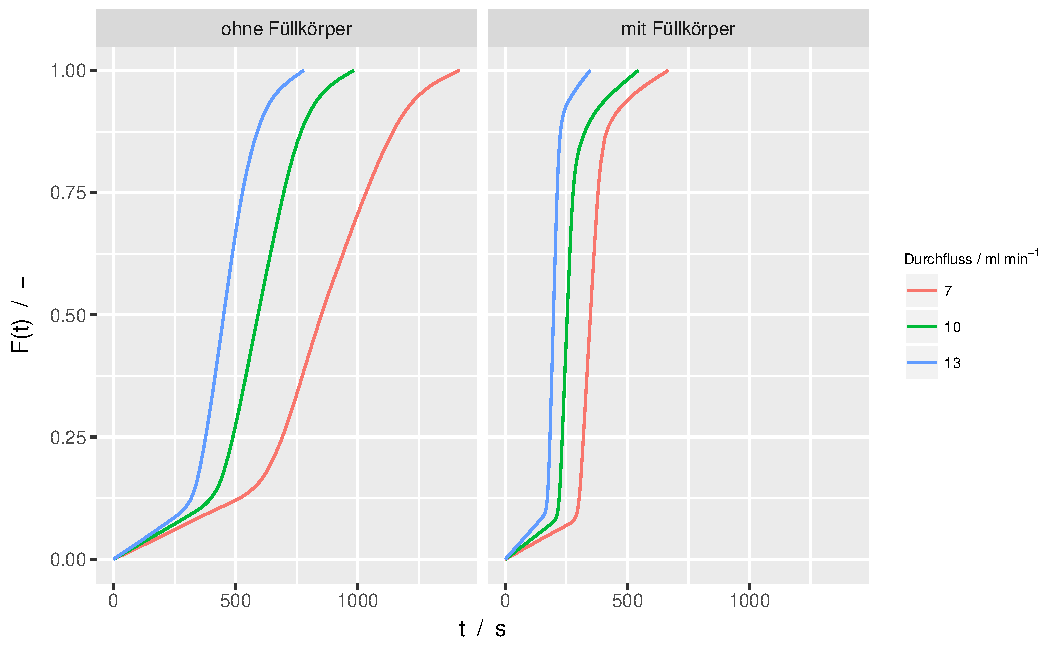
\includegraphics[width=1\textwidth]{Graphics/F_stoss.pdf}
\caption[Verweilzeitsumme Stoßmarkierungen]{Verweilzeitsummen aus der Stoßmarkierung}
\label{summe_stoss}
\end{figure}
\noindent

In Abbildung \ref{summe_stoss} zeigt sich zu Beginn der Kurve ein untypisches lineares Verhalten. Dies besitzt einen mathematischen Hintergrund. Gemessen wird eine sehr kleine Grundleitfähigkeit, was einer speziellen Konzentration entspricht. Diese Konzentration wird in der Verweilzeitsummenverteilung nummerisch aufsummiert und ergibt so den linearen Verlauf am Anfang der Kurve. Ansonsten zeigt sich ein ähnliches Bild wie im E(t) verlauf. Der Versuch im ersten Reaktor mit dem niedrigsten Durchfluss zeigt eine größere Verweilzeit als beispielsweise mit $13\,\text{ml}\cdot\text{min}^{-1}$.

\subsection{Normierte Verweilzeitdichtefunktion $E(\theta)$}

Unter Einbindung der dimensionslosen Verweilzeit $\theta$ bzw. der mittleren Verweilzeit $\bar{t}$ kann die normierte Verweilzeitsummenfunktion bestimmt werden. Die Integrale der mittleren Verweilzeit können ebenfalls diskretisiert ausgedrückt werden. Die Berechnung ist im Folgenden dargestellt:

\begin{align}
E(\theta_i) =&\; E(t_i) \cdot \bar{t} \\
\text{mit }\theta_i=&\;\frac{t_i}{\bar{t}}\\
\text{und }\bar{t} = &\;\frac{\int_{0}^{\infty}t_i\cdot c_i \cdot\text{d}t_i}{\int_{0}^{\infty}c_i \cdot\text{d}t_i} \approx \frac{\sum t_i\cdot c_i \cdot \Delta t_i}{\sum c_i \cdot \Delta t_i} \\
\notag
\end{align} 
\noindent
Die Summe von $\sum c_i \cdot \Delta t_i$ wurde zuvor berechnet. Für $\sum t_i\cdot c_i \cdot \Delta t_i$ ergibt sich für der unten berechnete Wert. Des Weiteren lässt sich anschließend $\bar{t}$ und $E(\theta)$ ($t= 640\,s$) für den ersten Versuch im ersten Reaktor berechnen:

\begin{align*}
\sum t_i\cdot c_i \cdot \Delta t_i =&\;t_1\cdot c_1 \cdot \Delta t_1 + t_2\cdot c_2 \cdot \Delta t_2+\;...\,+t_n\cdot c_n \cdot \Delta t_n \\
\sum t_i\cdot c_i \cdot \Delta t_i =&\; 3\,\s\cdot 0,0014\,\frac{\mole}{\litre}\cdot 3\,\s + 6\,\s\cdot 0,0014\,\frac{\mole}{\litre}\cdot 3\,\s+\;...\\
&...\;+ 1416\,\s\cdot 0,0013\,\frac{\mole}{\litre}\cdot 3\s \approx 4912,0634\,\frac{\mole\cdot\s^2}{\litre}\\
\bar{t} =&\; \frac{4916,676\,\frac{\mole\cdot\s^2}{\litre}}{5,91\,\frac{\mole\cdot\s}{\litre}} \approx 831,9\,\s\\
E(\theta_{864\,\s}) =&\; E(864\,\s)\cdot\bar{t} = 0,0015\,\frac{1}{\s} \cdot 831,9\,\s \approx 1,2479\\
\end{align*} 


\begin{figure}[H]
\centering
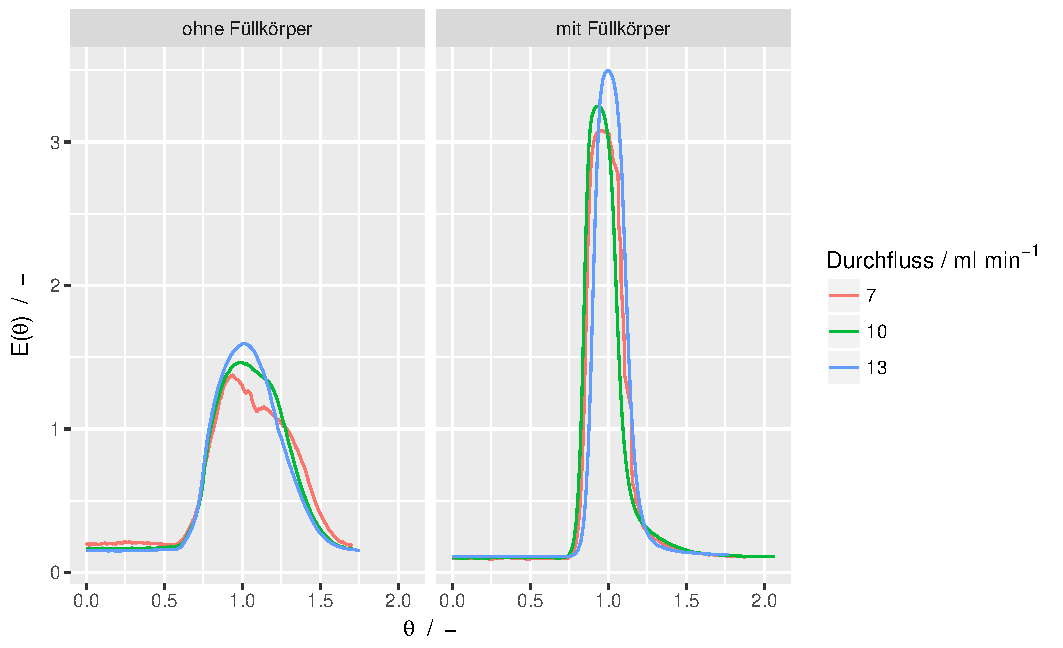
\includegraphics[width=1\textwidth]{Graphics/E_theta_stoss.pdf}
\caption[Normierte Verweilzeitdichte Pulsmarkierungen]{Normierte Verweilzeitdichten aus der Pulsmarkierung}
\label{dichte_stoß_norm}
\end{figure}
\noindent

Wie zu sehen ist werden durch $\theta$ die Kurven auf einen einheitlichen Wert gebracht und lassen sich im Bezug auf die Größe des Peaks besser interpretieren. Zu sehen ist das der Peak mit dem meisten Durchfluss am größten ist, sowohl beim Ersten als auch beim Zweiten Reaktor. Dies ist auf die Schnelligkeit des Tracers durch den Reaktor zurückzuführen, da die Fläche unter der Kurve 1 ist.

\subsection{Berechnung der Standardabweichung und des Dispersionsgrades}

Letztendlich lässt sich aus allen Informationen, die durch den Versuch generiert werden können, die Standardabweichung $\sigma^{2}_t$, standardisierte Standardabweichung $\sigma^{2}_\theta$ und die Bodenstein-Zahl $Bo$ errechnet, welche ein Maß für die Dispersion und somit axiale Rückvermischung im betreffenden Reaktor ist. Durch Diskretisierung kann das Integral abermals numerisch gelöst werden:

\begin{align}
\sigma^{2}_t =&\;\frac{\int_{0}^{\infty}(t_i-\bar{t})^2\cdot c_i \cdot\Delta t_i}{\int_{0}^{\infty}c_i\cdot\Delta t_i} \approx \frac{\sum t_{i}^2\cdot c_i \cdot\Delta t_i}{\sum c_i\cdot\Delta t_i} - \bar{t}^2\\
\sigma_\theta^2 =&\;\frac{\sigma^{2}_t}{\bar{t}^2}\\
\text{Bo} =&\; \frac{2}{\sigma_\theta^2}\\
\sum t_{i}^2\cdot c_i \cdot\Delta t_i =&\; t_{1}^2\cdot c_1 \cdot\Delta t_1 + t_{2}^2\cdot c_2 \cdot\Delta t_2+\;...\;+t_{n}^2\cdot c_n \cdot\Delta t_n \\
\sum t_{i}^2\cdot c_i \cdot\Delta t_i =&\; 9\,\s^2\cdot 0,0014\,\frac{\mole}{\litre} \cdot 3\,\s + 36\,\s^2\cdot 0,0014\frac{\mole}{\litre} \cdot \s+\;...\nonumber\\\notag
&...\;+ 2005056\;\s^2\cdot 0,0013\;\frac{\mole}{\litre} \cdot 3\;\s \approx 4590635\,\frac{\mole \cdot \s^3}{\litre}\notag
\end{align}

Für die beispielhaften Parameter errechnet sich:

\begin{align*}
\sigma^{2}_t =&\;\frac{ 4590635,0\,\frac{\mole \cdot \s^3}{\litre}}{ 5,91\frac{\mole \cdot \s}{\litre}} - 692107,19
\,s^2\approx 84654,55
s^2\\
\sigma_\theta^2 =&\; 84654,55\,\frac{\s^2}{692107,19\,\s^2}\approx 0,12\\
\text{Bo} =&\; \frac{2}{0,1223}\approx 16,35
\end{align*}

Die berechneten Parameter für alle Versuche der Pulsfunktion sind in Tabelle \ref{tab:werte_pulse} aufgelistet.

\begin{table}[H]
  \centering
  \caption{Ergebnisse der Pulsfunktion}
    \begin{tabular}{ccccccc}
    \toprule
    Versuch & Reaktor & Durchfluss / ml\,min$^{-1}$ & $\bar{t}$ / s & $\sigma_t^2$ / s$^2$ & $\sigma_{\theta}^2$ / - & $Bo$ / - \\
    \midrule
    
    1     & ohne Füllk. & 7     & 831,93 & 84654,55 & 0,12  & 16,35 \\
    2     & ohne Füllk. & 10    & 577,63 & 34642,39 & 0,10  & 19,26 \\
    3     & ohne Füllk. & 13    & 444,85 & 19696,53 & 0,10  & 20,09 \\
    4     & mit Füllk. & 7     & 354,03 & 8713,79 & 0,07  & 28,77 \\
    5     & mit Füllk. & 10    & 263,47 & 6292,53 & 0,09  & 22,06 \\
    6     & mit Füllk. & 13    & 195,97 & 2402,18 & 0,06  & 31,97 \\
    \bottomrule
    \end{tabular}%

  \label{tab:werte_pulse}%
\end{table}%

\newpage

\section{Stufenfunktion}

Die Stufenfunktion wird zur Ermittlung der Verweilzeitverteilung verwendet indem die NaCl-Lösung durch den Reaktor gepumpt wird und die Leitfähigkeit der austretenden Lösung gemessen wird. Die Stufenfunktion wird auch als Verdrängungsmarkierung bezeichnet, da die nicht leitfähige Grundlösung durch die leitfähige Wasserlösung verdrängt wird und das Maximum der Stufenfunktion erreicht wird, sobald die Leitfähigkeit der Wasserlösung am Reaktoraustritt detektiert wird. Folglich wird als erster Schritt in der Auswertung nicht die Verweilzeitdichteverteilung sondern die Verweilzeitsummenverteilung F(t) berechnet. Als Resultat dieses Unterschiedes folgen die Berechnungen der Verweilzeitverteilung zwar denselben Gleichungen als jene mit der Pulsfunktion, aber einem anderen Schema, auf welches in folgenden Punkten genauer eingegangen wird. Die Berechnungen werden für den 7. Versuch durchexerziert (siehe Tabelle \ref{tab:Versuchsnummerierung}). Die dazu notwendigen Gleichungen sind aus Quelle \cite{Skript_2018,Chem_Reaktion_2018} entnommen.

\subsection{Verweilzeitsummenfunktion F(t)}

Das Ergebnis der Verdrängungsmarkierung liefert eine S- bzw. Sigmoidale- Kurve im Konzentrations-Zeit-Diagramm. Diese Kurve wird in die Verweilzeitsummenverteilung umgerechnet. Sie beschreibt den Anteil der Konzentration, die gemessen wird, im Verhältnis zur effektiven maximalen Konzentration. Die maximale Konzentration ergibt sich aus den Messungen. Sobald sich eine stationäre Konzentration einstellt, wird der Versuch beendet. Diese stationäre Konzentration kann somit als $c_{max}$ definiert werden. 

\begin{align}
F(t_i)=&\;\frac{c_i(t_i)}{c_{max}}\\
\end{align}

Für die Abbildung der Verweilzeitsummenverteilung müssen anschließend die einzelnen Werte für $F(t)$ addiert werden. Für die 332 Sekunde ergibt sich beispielsweise:

\begin{equation}
F(332\,s)=\,\frac{ 0,0001\,\frac{\mole}{\litre}}{0,0110\,\frac{\mole}{\litre}} \approx 0,0104 \notag
\end{equation}
\noindent
In Abbildung \ref{summe_step} ist die Verweilzeitsumme aus der gemessenen Stufenfunktion für die Versuche 7-12 dargestellt.

\begin{figure}[H]
\centering
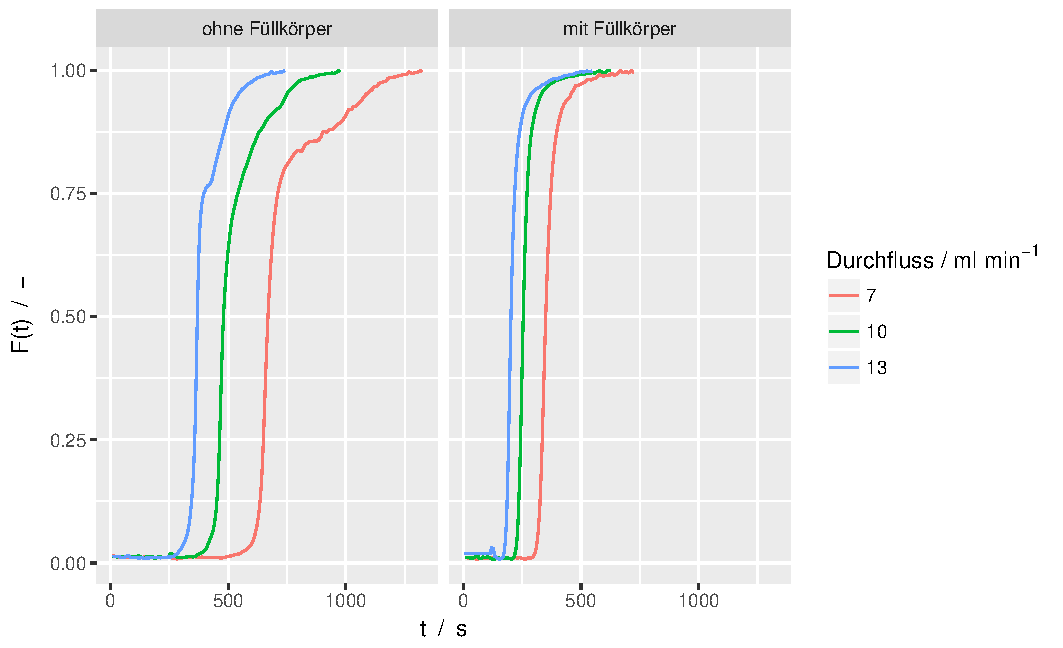
\includegraphics[width=1\textwidth]{Graphics/F_step.pdf}
\caption[Verweilzeitsumme Sprungfunktion]{Verweilzeitsummen aus der Stufenfunktion}
\label{summe_step}
\end{figure}
\noindent

\subsection{Verweilzeitdichteverteilung E(t)}

Die Verweilzeitdichteverteilung kann durch Ableiten der Verweilzeitsummenverteilung kalkuliert werden. Unter Anwendung diskreter Zeitschritte $\Delta t$ und Werten für $\Delta F (t)$ ergeben sich folgende Werte:

\begin{align}
E(t_i)=&\; \frac{\Delta F(t_i)}{\Delta t_i}= \frac{F(t_{i})-F(t_{i-1})}{t_i-t_{i-1}}\\
E(332\,\s)=&\; \frac{0,0104
 - 0,0105}{332\,\s - 329\,\s} = -0,00002\,\frac{1}{s}\notag \text{ (Rauschen)}
\end{align}

Der negative Wert für E(t) ergibt sich daher, da zu diesem Zeitpunkt die Konzentration in kleinen Schritten steigt und wieder sinkt und folglich die Verweilzeitsummenfunktion keine positive Steigung hat und damit die numerische Ableitung negativ wird. Es ist an dieser Stelle relevant zu erwähnen, dass bei allen Berechnungen zum Glätten der Konzentrationsverläufe und der daraus resultierenden Verläufe ein gleitender Mittelwert mit vier Werten pro Berechnung verwendet wird.
%\todo{Rauschen beschreiben}

In Abbildung \ref{dichte_step} ist die Verweilzeitdichtefunktion E(t) aus der Stufenfunktion bzw. Verdrängungsmarkierung dargestellt. 

\begin{figure}[H]
\centering
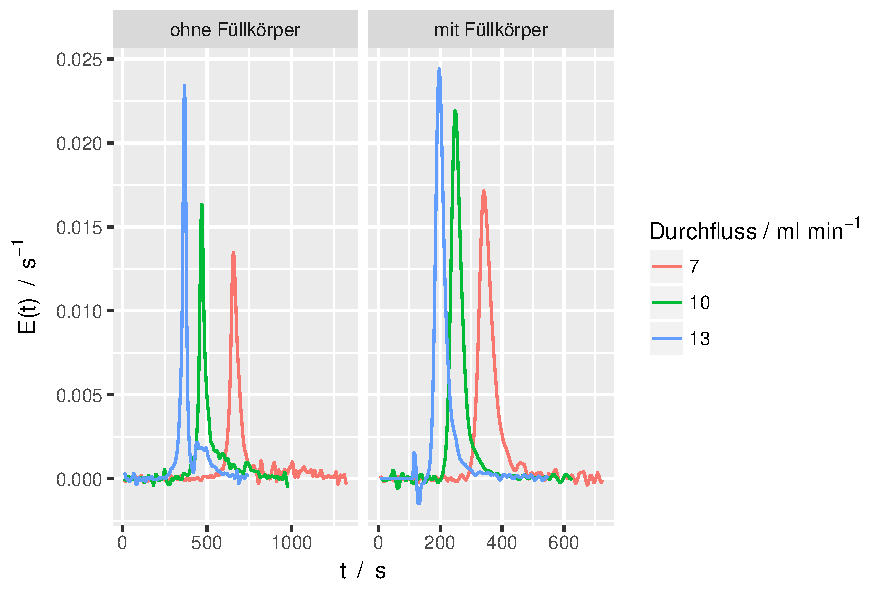
\includegraphics[width=1\textwidth]{Graphics/E_step.pdf}
\caption[Verweilzeitdichte Stufenfunktion]{Verweilzeitdichten aus der Stufenfunktion}
\label{dichte_step}
\end{figure}
\noindent

\subsection{Normierte Verweilzeitdichteverteilung $E(\theta)$}

Die Berechnung der standardisierten Verweilzeitdichteverteilung läuft analog zur Pulsverteilung ab. Lediglich die mittlere Verweilzeit errechnet sich durch eine andere Gleichung. Die Gleichung lässt sich wie folgt darstellen:

\begin{align}
\bar{t}=&\; \frac{\int_{0}^{c_{max}}t_i \cdot\text{d}c_i}{\int_{0}^{c_{max}}\text{d}c_i}\approx \frac{\sum t_i\cdot\Delta c_i}{\Delta c_{max}}\\
\sum t_i\cdot\Delta c_i =&\; t_1\cdot\Delta c_1 + t_2\cdot\Delta c_2+\;...\;+t_n\cdot\Delta c_n\\
\sum t_i\cdot\Delta c_i =&\; 12\,\s\cdot0\,\frac{\mole}{\litre}  + 15\,\s\cdot 0\,\frac{\mole}{\litre}+\;...\notag\\
&...\;+1322\,\s\cdot 0\,\frac{\mole}{\litre}\approx 7,9291\,\frac{\mole\cdot\s}{\litre} \notag
\end{align}

Für den ersten Versuch aus dem ersten Reaktor ohne Füllkörper ergibt sich folgende mittlere Verweilzeit:

\begin{equation}
\bar{t}= \frac{7,9291\,\frac{\mole\cdot\s}{\litre}}{0,011\,\frac{\mole}{\litre}} \approx 723,9\,\s\notag
\end{equation}
\noindent
Analog zur Pulsfunktion kann auch für die Stufenfunktion die berechnete Verweilzeitdichte mit der dimensionslosen Verweilzeit $\theta$ die normierte Verweilzeitdichte $E(\theta)$ ermittelt werden (siehe Abbildung \ref{dichte_step_norm}).


\begin{figure}[H]
\centering
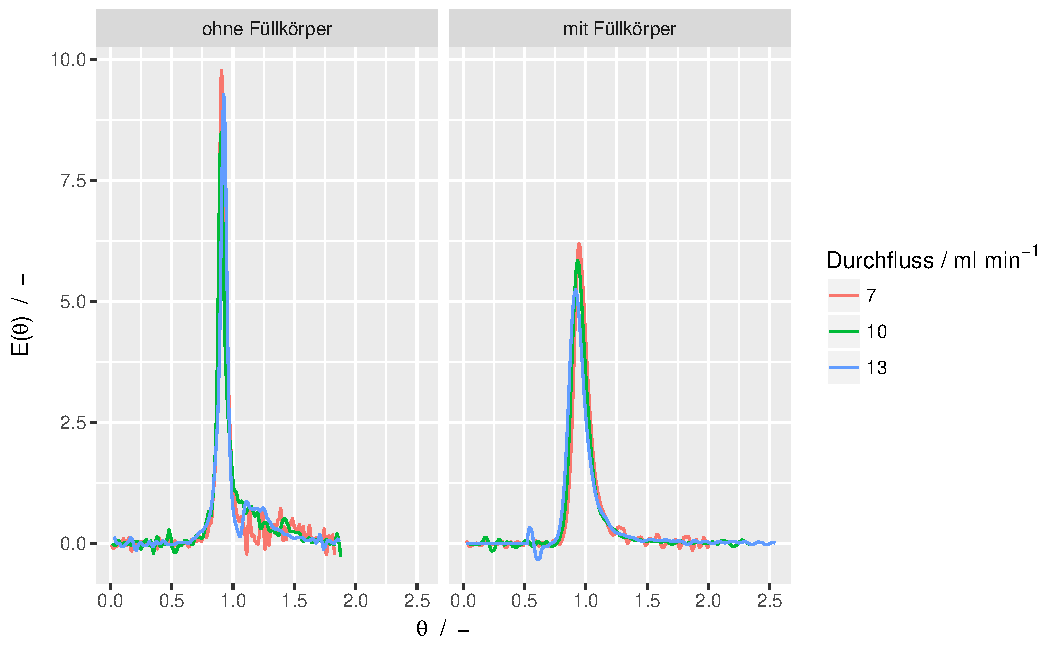
\includegraphics[width=1\textwidth]{Graphics/E_theta_step.pdf}
\caption[Normierte Verweilzeitdichte Stufenfunktion]{Normierte Verweilzeitdichten aus der Stufenfunktion}
\label{dichte_step_norm}
\end{figure}
\noindent


\newpage
\subsection{Berechnung der Standardabweichung und des Dispersionsgrades}

Die Bodenstein-Zahl und $\sigma_\theta^2$ errechnen sich analog zu Punkt 4.2.4. Zuvor wird $\sigma_t^2$ nach folgendem Schema errechnet: 
 
\begin{align}
\sigma_t^2=&\;\frac{\sum t_i^2\cdot\Delta c_i}{\Delta c_{max}} - \bar{t}^2\\
\sum t_i^2\cdot\Delta c_i =&\;t_1^2\cdot \Delta c_1 + t_2^2\cdot \Delta c_2 +\;...\;+t_n^2\cdot \Delta c_n\\
 \sum t_i^2\cdot\Delta c_i =&\;144\,\s^2 \cdot 0\,\frac{\mole}{\litre} + 225\,\s^2 \cdot 0\,\frac{\mole}{\litre}+\;...\notag\\\notag
&...\;+ 1747684\,\s^2 \cdot 0\frac{\mole}{\litre}\approx 5999,054\,\frac{\mole\cdot\s^2}{\litre}\\\notag
 \sigma_t^2=&\;\frac{5999,054\,\frac{\mole\cdot \s^2}{\litre}}{0,011\,\frac{\mole}{\litre}} - 524033,4\,\s^2 \approx 23658,87\,\s^2\\\notag
\end{align}
\noindent

Die Ergebnisse der einzelnen Versuche sind in Tabelle \ref{tab:werte_step} aufgelistet

\begin{table}[H]
  \centering
  \caption{Ergebnisse der Stufenfunktion}
    \begin{tabular}{ccccccc}
    \toprule
    Versuch & Reaktor & Durchfluss / ml\,min$^{-1}$ & $\bar{t}$ / s & $\sigma_t^2$ / s$^2$ & $\sigma_{\theta}^2$ / - & $Bo$ / - \\
    \midrule
    7     & ohne Füllk. & 7     & 723,90 & 23658,87 & 0,05  & 44,30 \\
    8     & ohne Füllk. & 10    & 519,47 & 11061,50 & 0,04  & 48,79 \\
    9     & ohne Füllk. & 13    & 395,90 & 5459,75 & 0,03  & 57,42 \\
    10    & mit Füllk. & 7     & 361,04 & 2975,48 & 0,02  & 87,62 \\
    11    & mit Füllk. & 10    & 266,66 & 2144,40 & 0,03  & 66,32 \\
    12    & mit Füllk. & 13    & 215,01 & 2407,54 & 0,05  & 38,40 \\
    \bottomrule
    \end{tabular}%

  \label{tab:werte_step}%
\end{table}%

\newpage

\section{Vergleich der experimentell ermittelten Verteilungen}



Abbildung \ref{dichte_stoss} zeigt die experimentell ermittelten Verweilzeitdichten mit der Pulsfunktion. Links ist Reaktor 1 (ohne Füllkörper) und rechts ist Reaktor 2 (mit Füllkörper) dargestellt.  Es wird gezeigt, dass sich bei niedrigeren Durchflüssen eine niedrigere Verweilzeitdichte einstellt (niedrigere Peaks). Dies resultiert daraus, dass der Tracer generell mehr Zeit benötigt um die Reaktor zu passieren. Bei dem Reaktor ohne Füllkörper werden grundsätzlich bei allen Versuchen deutlich niedrigere Verweilzeitdichten als bei dem bepackten Reaktor berechnet. Sie sind niedriger, weil der Reaktor ein größeres Füllvolumen besitzt und somit der Tracer bei gleichem Volumenstrom länger im Reaktor verweilt. Eine größere Verweilzeit in dem Reaktor bedeutet mehr Zeit für Rückvermischungen, was die Breite der geplotteten Peaks erhöht. Der parabolische Strömungsverlauf in den Rohrreaktoren begünstigt eine Rückvermischung des Tracers. Weiters lässt sich feststellen, dass bei dem Versuch mit 7\,$\text{ml}\cdot\text{min}^{-1}$ in dem Reaktor ohne Packung bei circa 900\,s eine Abweichung des Trends festzustellen ist. Es kann angenommen werden, dass dies aufgrund einer Luftblase auftritt, die durch den Reaktor zum Detektor transportiert wurde und so die Messung verfälscht. Schlussendlich ist gezeigt, dass je geringer die Verweilzeit im Reaktor ist, desto höher und desto schmäler sind die Verweilzeitdichtepeaks des Tracers. 
\\
\\
Abbildung \ref{dichte_step} zeigt die Verweilzeitdichtefunktion der Experimente mit der Stufenfunktion. Links ist der Reaktor ohne Packung und rechts ist der Reaktor mit Packung abgebildet. So wie in Abbildung \ref{dichte_stoss} ist auch hier ersichtlich, dass niedrigere Durchflüsse niedrigere Peaks erzeugen. Es fällt jedoch auch auf, dass die Abweichung des Reaktors geringer ist als bei den Versuchen mit der Pulsfunktion. Dies lässt sich zurückführen auf die unterschiedliche Bestimmungsmethode der Verweilzeit-Verteilungen mittels Puls- oder Stufenfunktion, da bei der Bestimmung mittels Pulsfunktion die geringere Konzentration des in geringen Mengen injiziierten Tracers (0,4\,ml) auf Rückvermischung bzw. Dispersion sensibler reagiert als bei der Stufenmarkierung in welcher im Endeffekt ein größeres Volumen zur Messung zur Verfügung steht. Es wird zwar die Verweilzeitdichteverteilung verglichen, der genannte Fehler der Konzentration wird aber über die rechnerische Bestimmung der Verweilzeitdichteverteilung mitgezogen. Vergleicht man die beiden Markierungsfunktionen mit einander, zeigt sich, dass bei der Pulsfunktion das Füllvolumen des Reaktors einen größeren Einfluss auf die Verweilzeitdichteverteilung hat als bei der Stufenfunktion. 

\newpage

\section{Beschreibung der Verweilzeitsummenfunktion mit dem Kaskadenmodell}
\label{sec:kaskade}


Ein Rohrreaktor verhält sich im idealen Fall wie eine Rührkesselkaskade, sprich eine Serienschaltung von Rührkesseln mit der Anazhl an $N$ Rührkesseln. Geht die Anzahl der Rührkessel gegen unendlich $N \rightarrow \infty$, ist das Verhalten eines idealen Rohrreaktors ersichtlich. Im realen Fall wird daher das ideale Strömungsrohr durch eine bestimmte Anzahl an Rührkesseln angenähert. Im Folgenden wird die Verweilzeitsummenfunktion für alle Versuche aus dem Kaskadenmodell generiert. Die äquivalente Anzahl an Rührkesseln nach dem Kaskadenmodell wird über $E_{\theta,max}$ laut \cite{Skript_2018} berechnet:

\begin{align}
&N = -1,762 + 0,569\cdot E_{\theta,max} + 6,206\cdot (E_{\theta,max})^2
\end{align}

Für den 1. Versuch ist $E_{\theta,max} = 1,375$. Somit gilt für $N$:

\begin{align*}
N = -1,762 + 0,569\cdot 1,375 + 6,206\cdot 1,375^2 = 10,75 \;\widehat{=}\;11\,\text{Rührkessel}\\
\end{align*}
Anschließend wird nach dem Kaskadenmodell die Verweilzeitsummenverteilung für die berechnete Anzahl an Rührkesseln erzeugt. Dabei kann F(t) im Kaskadenmodell mit dem folgenden Modell bestimmt werden \cite{Chem_Reaktion_2018}:

\begin{align}
c_{i,N}^{aus}=c_{i,N}^{ein} \cdot &\left(1-\text{exp}\left(-N\cdot\frac{t}{\tau}\right) \cdot \sum\limits_{n = 1}^N\frac{1}{(n-1)!}\cdot\Bigl(N\cdot\frac{t}{\tau}\Bigr)^{n-1}\right) \\
&\text{wobei } \frac{c_{i,N}^{aus}}{c_{i,N}^{ein}}= \frac{c_i(t_i)}{c_{max}}=F(t_i)\nonumber\\
&\text{und } \tau = \bar{t}\notag
\end{align}

Damit ergibt sich für eine Anzahl von N=11 Rührkessel folgender Wert zum Zeitpunkt $t$:

\begin{align*}
F(t)=&1-\text{exp}\left(-11\cdot\frac{t}{831,93\,\s}\right) \cdot \biggl(1+11\cdot\frac{t}{831,93\,\s} + \frac{1}{2!}\cdot \Bigl(11\cdot\frac{t}{831,93\,\s}\Bigr)^2 +\;...\\
&...\;+\frac{1}{10!}\cdot\Bigl(11\cdot\frac{t}{831,93\,\s}\Bigr)^{10} \biggr) \notag
\end{align*}

Die Berechnung von $F(t)$ erfolgt exemplarisch für $t = 503\,\s$:

\begin{align*}
F(t)=&1-\text{exp}\left(-11\cdot\frac{503\,\s}{831,93\,\s}\right) \cdot \biggl(1+11\cdot\frac{503\,\s}{831,93\,\s} + \frac{1}{2!}\cdot \Bigl(11\cdot\frac{500\,\s}{831,93\,\s}\Bigr)^2 +\;...\\
&...\;+\frac{1}{10!}\cdot\Bigl(11\cdot\frac{503\,\s}{831,93\,\s}\Bigr)^{10} \biggr) = 0,0753 \notag
\end{align*}

Wird nun aus der Summenverteilung die Dichtverteilung gebildet (siehe Kapitel 4.3.2) und anschließend eine neue Kurve für $E(\theta)$ erzeugt, kann ein neues $E_{\theta,max}$ abgelesen bzw. bestimmt werden. Dies liefert eine neue Anazhl an Rührkesseln und weiters eine neue Summenverteilung. Durch dieses iterative Vorgehen wird die Kurve angenähert und die optimale Anzahl an $N$ ermittelt, welche das reale Strömungsrohr am Besten beschreibt. Die Ergebnisse dieses Vorgehens sind im Folgenden in Tabelle \ref{tab:kaskade} und Abbildung \ref{F_kaskade} dokumentiert bzw. zusammengefasst.

\begin{table}[H]
\centering
\caption{Versuchsnummerierung mit Versuchsparametern}
     \begin{tabular}{c|cc|cc|cc}
     \toprule
    \multirow{2}[1]{*}{\#} & \multicolumn{2}{c|}{experimentelle Daten} & \multicolumn{2}{c|}{1. Iteration} & \multicolumn{2}{c}{2. Iteration} \\
          & $E_{\theta,max}$ & $N$     & $E_{\theta,max}$ & $N$ & $E_{\theta,max}$ & $N$ \\
    \midrule
    1     & 1,3752 & 10,7576 & 1,3762 & 10,7746 & 1,3762 & 10,7746 \\
    2     & 1,4653 & 12,3965 & 1,4867 & 12,8018 & 1,4867 & 12,8018 \\
    3     & 1,5954 & 14,9416 & 1,5897 & 14,8266 & 1,5897 & 14,8266 \\
    4     & 3,0823 & 58,9518 & 3,0733 & 58,6026 & 3,0733 & 58,6026 \\
    5     & 3,2498 & 65,6287 & 3,2593 & 66,0173 & 3,2833 & 67,0084 \\
    6     & 3,4984 & 76,1806 & 3,5171 & 77,0073 & 3,5395 & 78,0021 \\
    7     & 9,7700 & 596,1774 & - & - & - & - \\
    8     & 8,4866 & 450,0353 & - & - & - & - \\
    9     & 9,2687 & 536,6654 & - & - & - & - \\
    10    & 6,1895 & 239,5135 & - & - & - & - \\
    11    & 5,8450 & 213,5849 & - & - & - & - \\
    12    & 5,2486 & 172,1849 & - & - & - & - \\
    \bottomrule
    \end{tabular}%
\label{tab:kaskade}
\end{table}
\noindent

Für die Versuche 7 bis 12 konnte die Berechnung nicht durchgeführt werden, da die Berechnung ab einer Rührkesselanzahl von 172 aufgrund des Fakultätausdruckes scheitert. Die hohe Anzahl an Rührkesseln für diese Versuche deutet daraufhin, dass die Reaktoren bei dieser Versuchsart ein ideales Strömungsrohr sehr gut beschreiben. Diese Vermutung wird in Kapitel \ref{sec:umsatz} bestätigt, da die Umsätze welche aus den Verweilzeitverteilungen dieser Versuche berechnet wurden mit den idealen Umsätzen übereinstimmen.

\begin{figure}[H]
\centering
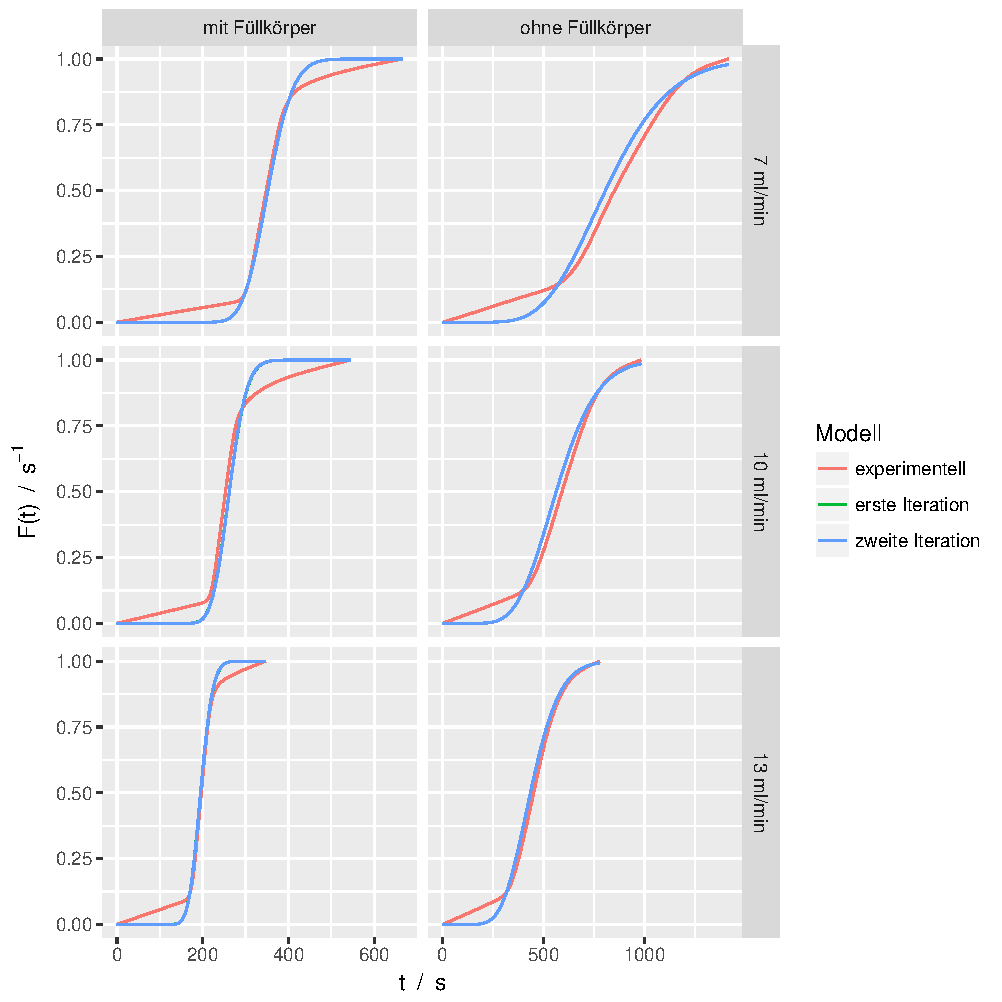
\includegraphics[width=1\textwidth]{Graphics/kaskade.pdf}
\caption[Reaktor mit CSTR-Kaskade modelliert]{Verweilzeitsummen: experimentelle Daten und CSTR-Kaskade im Vergleich}
\label{F_kaskade}
\end{figure}
\noindent

Für die Pulsfunktionsversuche konnten sinnvolle Werte für die Anzahl an Rührkesseln ermittelt werden. Bei den Versuchen 5 und 6 ändert sich die Anzahl der Rührkesseln in der Kaskade bei mehrmaligem iterieren geringfügig, bei den anderen Versuchen bleibt sie konstant. Der experimentelle und die berechneten Verweilzeitsummenverläufe sind in Abbildung \ref{F_kaskade} dargestellt. Die Kurven für die erste und zweite Iteration sind praktisch ident. Die Plots zeigen, dass sich die Reaktoren sehr gut durch eine Rührkesselkaskade beschreiben lassen.



\section{Reale VWZ-Verteilung im Vergleich mit idealen Reaktoren}

Stellt man nun zwischen den real ermittelten Verweilzeit-Verteilungen und dem idealen Verhalten eines Rohrreaktors, eines Rührkessels und einer Rührkesselkaskade, einen Vergleich an, muss zuallererst das ideale Verhalten definiert werden \cite{Skript_CVT_MCI}.  
\\
\\
Der ideale Rührkessel (\underline{C}ontinuously \underline{S}tirred \underline{T}ank \underline{R}eactor CSTR) wird im idealen Fall über die folgenden Gleichungen charakterisiert:

\begin{equation}
E(t) = \frac{1}{\bar{t}} \cdot \exp\left(-\frac{t}{\bar{t}}\right)
\end{equation}

\begin{equation}
F(t) = 1 - \exp\left(-\frac{t}{\bar{t}}\right)
\end{equation}
\noindent
\\
Das ideale Strömungsrohr (\underline{P}lug \underline{F}low \underline{R}eactor PFR) wird, wie der Name bereits impliziert, durch eine Propfenströmung charakterisiert. Sprich, ein Volumen das am Reaktoreingang eingebracht wird, wird nachdem es den Reaktor durchlaufen hat mit der Anfangskonzentration am Ausgang in einem sehr geringen Zeitfenster detektiert. Dadurch ergibt sich für die Verweilzeitdichteverteilung ein einmaliger Wert von 1 bei der hydraulischen Verweilzeit $\tau$ und eine Signumsfunktion für die Verweilzeitsummenfunktion, welche ab der hydraulischen Verweilzeit den Wert 1 einnimmt. 
\\
\\
Die ideale Rührkesselkaskade verhält sich abhängig von der Anzahl an Rührkesseln $N$ wie ein idealer Rührkessel ($N$ = 1 ) oder wie ein PFR ($N \rightarrow \infty$), da bei unendlicher Anzahl an Rührkesseln ein infinitesimales Volumenelement im Rohrreaktor ideal durchmischt wird und keine Akkumulation auftritt. Das Verhalten ist mit folgenden mathematischen Zusammenhängen beschreibbar. Die dazu notwendigen Gleichungen sind aus Quelle \cite{Skript_2018,Chem_Reaktion_2018} entnommen

\begin{equation}
E(t) = \frac{N \cdot (N \cdot t)^{N-1}}{\bar{t} \cdot (N-1)!} \cdot \exp\left(-N \cdot \frac{t}{\bar{t}}\right)
\end{equation}

\begin{equation}
F(t) = 1 - \exp\left(- N \cdot \frac{t}{\bar{t}}\right) \cdot \left[ \sum_{i=0}^{N-1} \left(\frac{1}{(i-1)!} \cdot \left(\frac{N \cdot t}{\bar{t}} \right)^i \right) \right]
\end{equation}
\noindent
\\
Im Folgenden sind die idealen Verläufe der Verweilzeitdichteverteilung (Abbildung \ref{dichte_vergleich}) und der Verweilzeitsummenfunktion (Abbidung \ref{summe_vergleich}) für den idealen CSTR, PFR und CSTR-Kaskade dargestellt.
\\
\\
\begin{figure}[H]
\centering
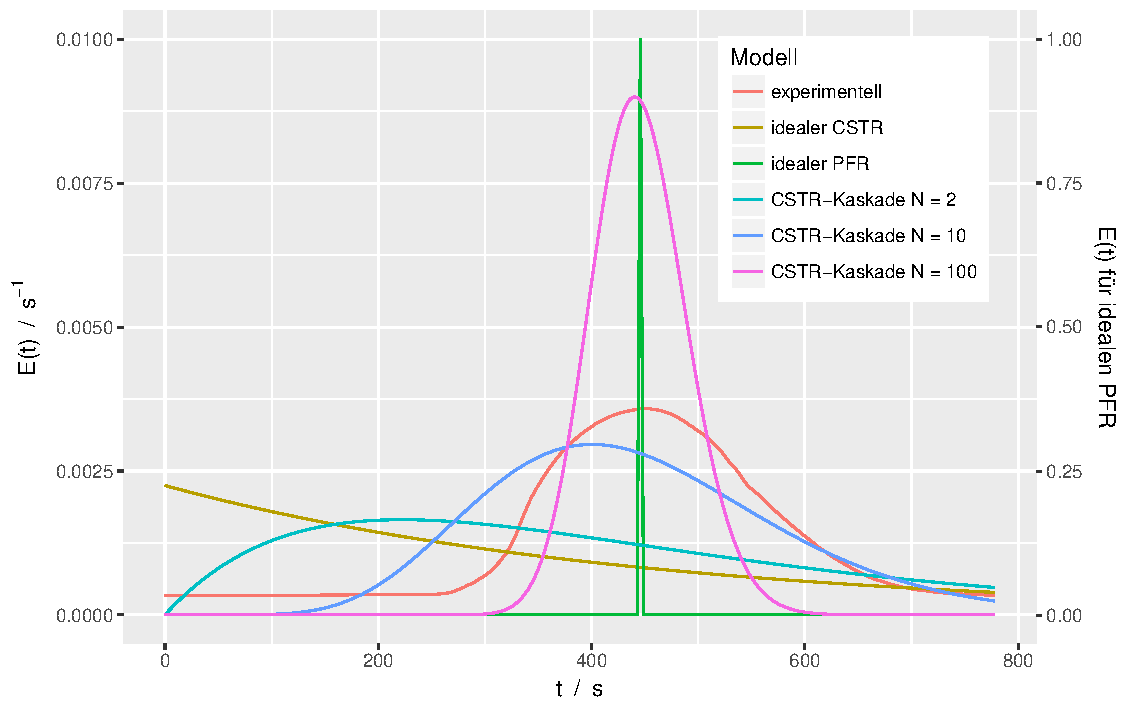
\includegraphics[width=1\textwidth]{Graphics/E_vergleich.pdf}
\caption[Vergleich Verweilzeitdichten]{Vergleich zwischen idealer und experimenteller Verweilzeitdichte}
\label{dichte_vergleich}
\end{figure}
\noindent

\begin{figure}[H]
\centering
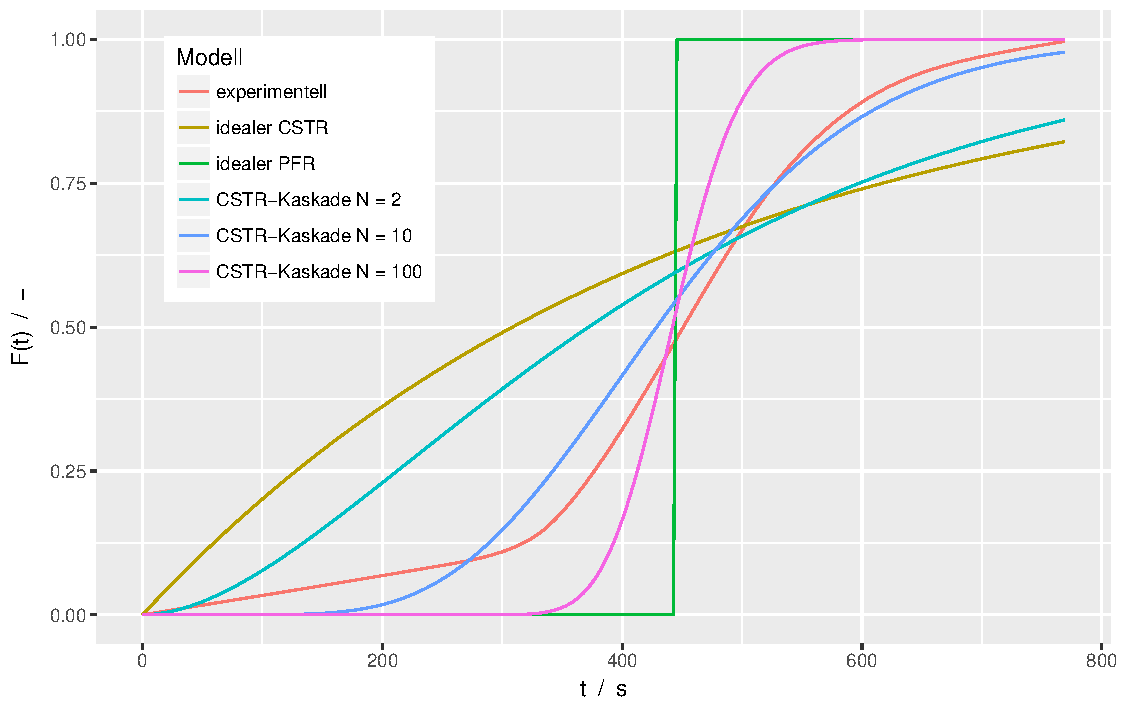
\includegraphics[width=1\textwidth]{Graphics/F_vergleich.pdf}
\caption[Vergleich Verweilzeitsummen]{Vergleich zwischen idealer und experimenteller Verweilzeitsummenverteilung}
\label{summe_vergleich}
\end{figure}
\noindent
\\
\\
Betrachtet man nun exemplarisch Versuch $#$3 (ohne Füllkörper, Pulsmarkierung, 13\,$\text{ml}\cdot\text{min}^{-1}$) in Abbildung \ref{dichte_vergleich}, erkennt man für die Verweilzeitdichteverteilung, dass das oben beschriebene Verhalten der Rührkesselkaskade mit steigender Anzahl an Rührkesseln dem Verhalten des PFRs immer ähnlicher wird. Zudem ist die Pfropfenströmung im PFR am engen Peak der Kurve gut erkennbar, da die hypothetische Konzentration an Tracer zu dem Zeitpunkt detektiert wird zu dem das Volumenelement den Reaktor durchlaufen hat und keine Rückvermischung auftritt. Die Abweichung der aus den Messdaten kalkulierten Verweilzeitverteilung im Realfall von den idealen Fällen lässt sich auf Strömungs-Nichtidealitäten wie Totzonen, Bypassströmungen und Kanalbildung, zurückführen, wobei die Kanalbildung in diesem Fall einen Bereich im Reaktor bezeichnet in welchem die Stromfäden einer Kurve folgen die ein schnelleres Durchlaufen des Reaktors zur Folge haben. An dieser Stelle kann ebenfalls erwähnt werden, dass durch das Aufwickeln des Rohrreaktors der " Dean-Effekt"' zum Tragen kommt \cite{Dean_Wirbel}. Durch das Aufwickeln spielen Zentrifugalkräfte eine Rolle, welche durch Geschwindigkeitsdifferenzen im Querschnitt des Rohres variieren. Diese Zentrifugalkräfte erzeugen Wirbel, sogenannte "Dean-Wirbel". Diese Wirbel verursachen eine axiale und radiale Durchmischung an der Stelle ihrer Entstehung und beeinflussen folglich die hydraulische Verweilzeit im Reaktor und die Konzentration welche am Ausgang gemessen werden kann. 
\\
\\
Eine weitere mögliche Ursache für die Nicht-Idealitäten bzw. Differenz der realen und theoretischen VWZ-Verteilungen liegt in der Pulsation des Förderstroms, wodurch das Messsignal verfälscht wird bzw. ein Volumenelement mit einer bestimmten Konzentration im Takt der Pumpe gefördert wird und somit beim Messen der Konzentration zwischen zwei Stößen der Pumpe eine andere Konzentration detektiert wird. 
\\
\\
Des Weiteren ist bei Betrachtung von de Abbildungen \ref{dichte_vergleich} und \ref{summe_vergleich} erkennbar, dass von den idealen Verläufen die Rührkesselkaskade mit $N$=10 am Besten in der Lage ist den experimentellen Verlauf zu beschreiben. Sprich, der analysierte Rohrreaktor kann in 10 ideale CSTRs mit gleichem Volumen aufgeteilt werden um dem realen Verhalten des Rohrreaktors am nächsten zu kommen. 
\newpage

\section{Anwendung des Compartmentmodells}

Dem Compartmentmodell liegt die Idee zu Grunde, dass sämtliche Nicht-Idealitäten der Verweilzeitverteilung eines realen Reaktors durch die Kombination von idealen Reaktoren und Totvolumina beschrieben werden können.
\par Zunächst wird das Gesamtvolumen der verwendeten Rohrreaktoren über den Innendurchmesser und der Rohrlänge bestimmt. Durch multiplizieren des jeweils verwendeten Volumenstroms mit der errechneten mittleren Verweilzeit wird das tatsächlich genutzte Volumen berechnet. Die Differenz der beiden Volumina entspricht dem von der Strömung nicht genutzten Totvolumen. Darin verbirgt sich aber auch die Volumenänderung des Schlauches durch die mit der Verwindung einhergehende Querschnittsänderung sowie – im Fall des gepackten Reaktors – das Volumen der Füllkörper.
\par Als nächster Schritt wird die Aufteilung des genutzten Volumens in das Volumen des idealen Rohrreaktors und des kontinuierlich Rührkessels ermittelt. Die Reihenfolge dieser beiden idealen Reaktoren ist bei der Auswertung der Verweilzeitverteilung nicht von Belangen. Es wird die Stufenfunktion eines idealen Rohrreaktors und eines kontinuierlichen Rührkessels auf die Verweilzeit $\tau$ umgeformt, addiert und wieder auf die Stufenfunktion umgeformt. Es ergibt sich:

\begin{equation}
F(t)_{fit} = 1 - \text{exp}\left[\frac{\tau_{PFR} - t_i}{\tau_{CSTR}}\right]
\end{equation}

\par Die Verweilzeiten in den einzelnen Compartments können über das Volumen und den Volumenstrom ausgedrückt werden, wobei das Volumen des kontinuierlichen Rührkessels als Differenz zwischen dem genutzten Gesamtvolumen und dem Volumen des Rohrreaktor-Compartments eingesetzt wird. So ergibt sich folgender Ausdruck:

\begin{equation}
F(t)_{fit} = 1 - \text{exp}\left[\frac{V_{PFR} - \dot{V} \cdot t}{\dot{V} \cdot {\bar{t}} - {V}_{PFR}}\right]
\end{equation}

Für den ersten Verusch (siehe S. \pageref{tab:Versuchsnummerierung}) errechnet sich beispielsweise folgender Wert bei $t$ = 661\,s:

\begin{equation}
F(661\,\s)_{fit} = 1 - \text{exp}\left[\frac{66\,\text{ml} - 7\,\frac{\text{ml}}{\text{min}}\cdot661\,\s }{7\,\frac{\text{ml}}{\text{min}}\cdot831,930\,\s - 66\,\text{ml}}\right] \approx 0,301
\end{equation}

\par Mithilfe eines Matlab-Files wird mit einer Schrittweite von 1\,ml das Volumen des Rohrreaktor -Compartments von 0 bis zum genutzten Gesamtvolumen variiert und jeweils die Fehlerquadratsumme zu den experimentellen Daten gebildet. Bei einer minimalen Fehlerquadratsumme entspricht die Volumenaufteilung von idealem Rohrreaktor und kontinuierlichem Rührkessel dem besten zu den Versuchsdaten passenden Compartmentmodell. In den nachfolgenden Abbildungen sind jeweils die Stufenfunktion der Versuchsdaten und des Compartmentmodell-Fits geplottet.

\par Die so bestimmten Aufteilungen der Compartments sind für jeden Versuch in Tabelle \ref{tab:compartment} dargestellt.

\begin{figure}[H]
\centering
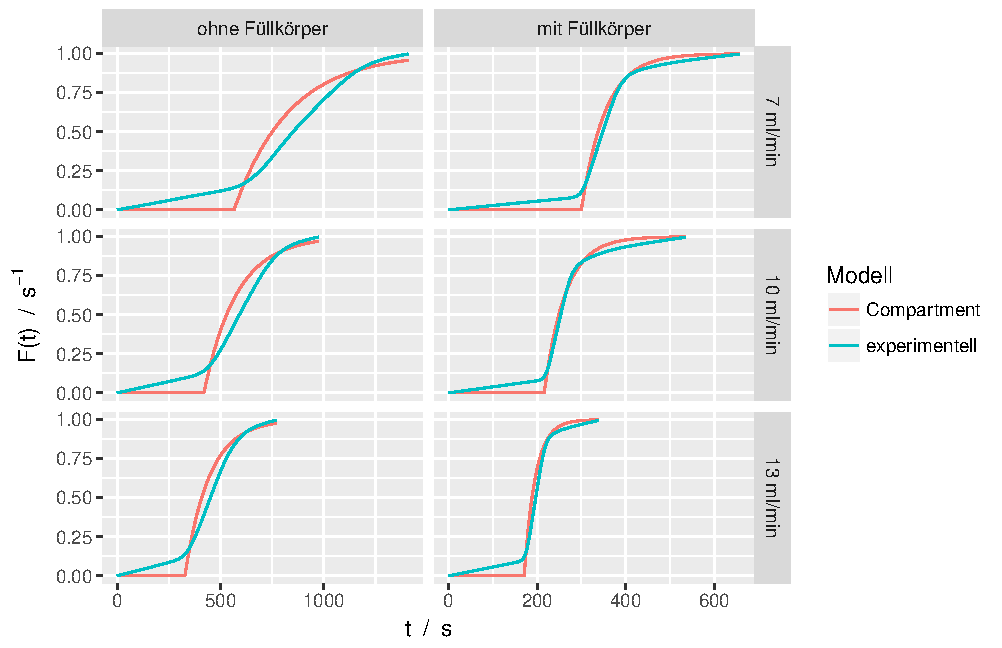
\includegraphics[width=1\textwidth]{Graphics/comp_stoss.pdf}
\caption[Compartment-Modell Stoßfunktion]{Summenverteilung für Compartment-Modell und experimentelle Daten - Pulsfunktion}
\label{fig:summe_comp_pulse}
\end{figure}
\noindent

\begin{figure}[H]
\centering
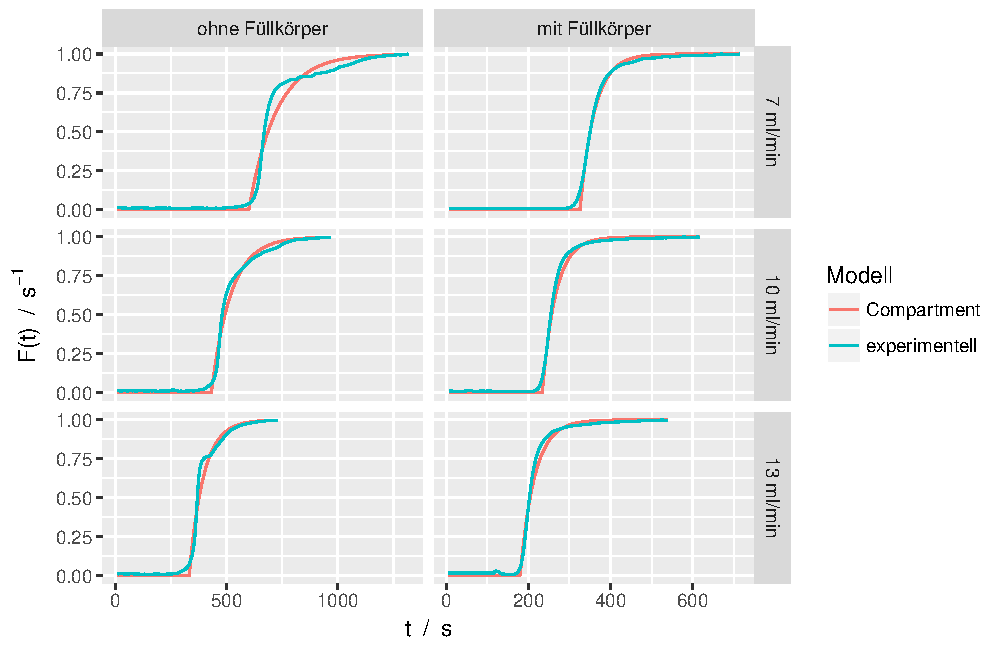
\includegraphics[width=1\textwidth]{Graphics/comp_step.pdf}
\caption[Compartment-Modell Sprungfunktion]{Summenverteilung für Compartment-Modell und experimentelle Daten - Stufenfunktion}
\label{fig:summe_comp_step}
\end{figure}
\noindent

\begin{landscape}

\begin{table}[C]
\centering
\caption{Ausgewertete Daten für das Compartment Modell}
\begin{tabular}{ccccccc}
\toprule 
Versuch $\#$ & Gesamtvolumen & Totvolumen & genutztes Volumen & Volumen PFR & Volumen CSTR & mittlere quadr. Abweichung des Fits \\
& in ml & in  ml & in ml & in ml & in ml & -\\
\midrule
1 & 98 & 1 & 97 & 66 & 31 & 0,0392 \\
2 & 98 & 2 & 96 & 70 & 26 & 0,0237 \\
3 & 98 & 2 & 96 & 70 & 25 & 0,0150\\
4 & 98 & 57 & 41 & 35 & 6 & 0,0096\\
5 & 98 & 54 & 44 & 36 & 8 & 0,0067\\
6 & 98 & 56 & 42 & 37 & 5 & 0,0092\\
7 & 98 & 14 & 84 & 70 & 14 & 0,0114\\
8 & 98 & 11 & 87 & 72 & 15 & 0,0031\\
9 & 98 & 12 & 86 & 72 & 14 & 0,0037\\
10 & 98 & 56 & 42 & 38 & 4 & 0,0018\\
11 & 98 & 54 & 44 & 39 & 5 & 0,0021\\
12 & 98 & 51 & 47 & 39 & 8 & 0,0027\\
\bottomrule
\end{tabular}
\label{tab:compartment}
\end{table}
\noindent

\end{landscape}



\par Die Daten der Versuche mit unterschiedlichen Volumenströmen jedoch gleichem Aufbau und gleicher Methode wurden gemittelt und folgende prozentuelle Auswertung erstellt.
\par Die ausgewerteten Stufenmodelle ergeben für den leeren Rohrreaktor ein gemitteltes Totvolumen von 12,5 \% des gesamten Reaktorvolumens, die Auswertung der Pulsfunktion ergab nur 1,5 \%. Aus der Stufenfunktion kann ein Anteil des kontinuierlichen Rührkessels am genutzten Volumen von 16,7 \% berechnet werden. Aus der Pulsfunktion wird ein Anteil von 28,6 \% berechnet.
\par Bei der Berechnung des gepackten Rohrreaktors wird bei der Auswertung der Stufenfunktion ein Totvolumen von 54,7 \% ermittelt. Die Auswertung der Pulsfunktion ergab 56,6 \%. Nach der Auswertung der Stufenfunktion können 12,9 \% des genutzten Volumens einem kontinuierlichen Rührkessel zugeordnet werden. Nach der Auswertung der Pulsfunktion beträgt der Anteil 15,4 \%.
\par Axiale Rückvermischung spielt diesen Berechnungen zu Folge bei beiden Reaktoren eine nicht zu vernachlässigende Rolle.

\newpage

\section{Berechnung der Bodenstein Zahl mit dem Dispersionsmodell}

Im Zuge des Laborpraktikums ist zu prüfen ob die Bodenstein-Zahl mit dem Dispersionsmodell berechenbar ist. Das Modell trifft für Bodenstein-Zahlen von Bo < 100 zu.
\\
\\
Dabei kann für Wertebereiche von $Bo$  das Verhalten eines Reaktors bzw. die Abweichung vom idealen Verhalten bezüglich dem Verhältnis von Konvektion zu Dispersion, beschrieben werden. Folgende Wertebereiche sind von Relevanz:


\begin{itemize}
    \item Bo < 100 mittlere Abweichung vom idealen Fließverhalten
    \item Bo < 1 starke Abweichung vom idealen Fließverhalten
    \item Bo > 100 geringe Abweichung vom idealen Fließverhalten 
\end{itemize}
\noindent
Das Maß der Abweichung ist als Verhältnis von Konvektion zu Dispersion zu verstehen, was der physikalischen Bedeutung der Bodenstein-Zahl entspricht \cite{fogler1999elements}. Grundsätzlichen stehen vier Möglichkeiten zur Verfügung um Bo < 100 zu berechnen, wobei sich diese Möglichkeiten durch die angewandten Randbedingungen unterscheiden. Diese Randbedingungen sind Kombinationen von entweder "'closed"' oder "'open'" Vessel (Kessel, Reaktor) und sind durch das Verhalten eines Reaktanden-Teilchens definiert, wobei beim closed Vessel ein Teilchen einer Pfropfenströmung folgt und den betrachteten Reaktorteil nur einmal passieren kann und beim open Vessel das betrachtete Teilchen den Reaktorteil mehrmals passieren kann und keine Pfropfenströmung sondern ein ähnliches Strömungsverhältnis zum Reaktoraus- bzw. -eingang vorhanden ist. Folgenden Gleichungen beschreiben laut \cite{Skript_2018} die diversen mathematischen Zusammenhänge zur Kalkulation der Bodenstein-Zahl mit den jeweiligen Randbedingungen.

\begin{enumerate}
    \item Closed-Closed Vessel
    \begin{equation}
        Bo_{cc} = \left(\frac{1}{\sigma_{\theta}^2 - 1}\right) + \sqrt{\left( \frac{1}{\sigma_{\theta}^2 - 1 \right) + \left( \frac{2}{\sigma_{\theta}} - 2 \right)}
    \end{equation}
    
    \item Open-Open Vessel
    \begin{equation}
        Bo_{oo} = \frac{1}{\sigma_{\theta}^2} + \sqrt{\left(\frac{1}{\sigma_{\theta}^2}\right)^2 + \left(\frac{8}{\sigma_{\theta}^2}\right)}
    \end{equation}
\end{enumerate}
\noindent
In Tabelle \ref{tab:BodensteinDispersion} sind die berechneten Bodenstein-Zahlen zusammengefasst, wobei $Bo$ ohne Index der Kalkulation mit der normierten Standardabweichung $\sigma_{\theta}^2$ entspricht. Als Randbedingungen werden closed-closed (Index $cc$) und open-open (Index $oo$) gewählt. Da $oo$ laut Literatur \cite{fogler1999elements,Skript_2018} am häufigsten dazu verwendet wird experimentelle Verläufe auszuwerten und die Auswertung mit $cc$ der Bodenstein-Zahl aus der Standardabweichung am nächsten kommt. Daher ist ersichtlich, dass die betrachteten Rohrreaktoren mit der $cc$ Randbedingung am Besten beschreibbar sind und eine Pfropfenströmung am Reaktorein- und -ausgang anzunehmen ist.


\begin{table}[H]
\centering
\caption{Berechnte Bodenstein-Zahlen mit unterschiedlichen Randbedingungen}
\begin{tabular}{cccc}
\toprule 
Experiment $\#$ & $Bo$ & $Bo_{cc}$ & $Bo_{oo}$\\
\midrule
1 & 16,35 & 15,29 & 19,68 \\
2 & 19,26 & 18,21 & 22,66 \\
3 & 20,09 & 19,04 & 23,51 \\
4 & 28,77 & 27,73 & 32,33 \\
5 & 22,06 & 21,02 & 25,52 \\
6 & 31,98 & 30,94 & 35,57 \\
7 & 57,06 & 56,05 & 60,82 \\
8 & 48,80 & 47,78 & 52,52 \\
9 & 44,29 & 43,27 & 47,98 \\
10 & 38,40 & 37,38 & 42,06 \\
11 & 66,09 & 65,07 & 69,87 \\
12 & 87,71 & 86,70 & 91,54 \\
\bottomrule
\end{tabular}
\label{tab:BodensteinDispersion}
\end{table}
\noindent

\newpage

\section{Reaktions-Umsatz Berechnung aus realem Verweilzeitverhalten}
\label{sec:umsatz}

Würde theoretisch eine Reaktion im Strömungsrohr ausgeführt werden, so beeinflusst das Verweilzeitverhalten des Reaktors den Umsatz der Reaktion im Sinne der mittleren Verweilzeit und dem  Strömungsverhalten durch Nicht-Idealitäten (Bypass, Totvolumen). Die Berechnung des Umsatzes hängt von der verwendeten Methode ab (Puls- oder Stufenfunktion), da sich die Verweilzeitdichtevereteilung auf eine andere Weise berechnen lässt. Als Reaktion mit weitgehend gut erforschter Kinetik wird die Veresterung von Essigsäure $CH_3COOH$ mit Methanol $CH_3OH$ zu Essigsäuremethylester $CH_3COOCH_3$ und Wasser $H_2O$ gewählt, welche laut Literatur \cite{Rolfe1934, mandake2013kinetic} mit einem Geschwindigkeitsgesetz zweiter Ordnung beschrieben werden kann.

\begin{equation*}
 CH_3COOH + CH_3OH \rightleftharpoons CH_3COOCH_3 + H_2O 
\end{equation*}
\noindent
Im weiteren Verlauf wird der Einfachheit halber die Reaktion mit folgenden Reaktanden referenziert und aufgrund des geringen Wertes der Reaktionsgeschwindigkeitskonstante der Rückreaktion eine irreversible Reaktion angenommen.

\begin{equation*}
    A + B \rightarrow C + D
\end{equation*}
\noindent
Die Kinetik wurde von Hinshelwood et. al und Mandake et. al \cite{Rolfe1934, mandake2013kinetic} erforscht und kann für 308\,K (unkatalysiert) mit der Reaktionsgeschwindigkeitskonstante $k$=1,5009 $\cdot  $10$^{-2}$\, $\litre\cdot\mole^{-1}\cdot\s^{-1}$ für die Hinreaktion beschrieben werden. Am Versuchstag wurde zwar nicht bei 309\,K hantiert. Dies sollte aber auf die Strömungseingenschaften von Wasser oder der NaCl-Lösung keine großen Einflüsse haben. Die Geschwindigkeitskonstante wird daher als passend aufgefasst. In einem nächsten Schritt muss die Anfangskonzentration $c_{A,0}$ definiert werden, welche im Verhältnis zur gemessenen Konzentration an NaCl-Tracer stehen kann, aber nicht muss, damit die gemessenen Werte der Leitfähigkeit bzw. Konzentration im Experiment für die Ermittlung des realen Umsatzes herangezogen werden können. Damit die Umsätze aber Werte erreichen die gut vergleichbar sind und nicht zu gering sind wird die Anfangskonzentration an Essigsäure $CH_3COOH$ mit $c_{A,0}$ = 2\,$\text{mol}\cdot\text{l}^{-1}$ definiert und für alle Versuche konstant gehalten. 
\\
\\
Das Geschwindigkeitsgesetz zweiter Ordnung und die Kalkulation des Umsatzes für den realen Fall ist im Folgenden dargestellt.

\begin{align}
\biggl(\frac{c_A}{c_{A,0}}\biggr)_{real} =&\; \int_{0}^{\infty} \biggl(\frac{{c}_A}{c_{A,0}}\biggr)_{Element} \cdot E(t)\cdot dt = (1-X_{real})\\
\biggl(\frac{{c}_A}{c_{A,0}}\biggr)_{Element} =&\; \frac{1}{1+k\cdot c_{A,0}\cdot t}\notag
\end{align}

Bei numerischer Lösung ergibt sich für die Reaktion somit folgender Umsatz für Versuch $\#$ 1:

\begin{align*}
 (1-X_{real}) =&\; \sum \biggl(\frac{{c}_A}{c_{A,0}}\biggr)_{ideal} \cdot E(t)\cdot \Delta t\\ \label{gl_Umsatz}
 (1-X_{real}) =&\; \sum \biggl(0,7355\biggr) \cdot 1,57\cdot 10^{-4} \cdot 3,01 + ... +  \biggl(0,0232 \biggr) \cdot 1,55 \cdot 10^{4} \cdot 3,01 \notag \\ 
 X_{real} =&\; 1 - 0,0543  \approx 0,95 \notag
\end{align*}
\noindent

Der ideale Umsatz berechnet sich wie folgt:

\begin{align}
 X_{ideal} =&\; 1 - \biggl(\frac{{c}_A}{c_{A,0}}\biggr)_{ideal} =\; \frac{1}{1+k\cdot c_{A,0}\cdot \bar{t}}\\
X_{ideal} =&\;1 - \frac{1}{1+ 0,015009\,\frac{\text{l}}{\text{mol}\,\text{s}}\cdot 2\,\frac{\text{mol}}{\text{l}}\cdot 831,93\,\text{s}}\nonumber\\
X_{ideal} =&\; 0,96\nonumber
\end{align}

Um die Nicht-Idealitäten der untersuchten Reaktoren mit dem Umsatz in Verbindung zu bringen werden die Umsätze im idealen und realen Fall für alle Versuche ermittelt. Die nach obigem Algorithmus ermittelten Umsätze sind in Tabelle \ref{tab:umsatz} gelistet.

\begin{table}[H]
\centering
\caption{Umsätze der Veresterungsreaktion ideal und real mit $k$ = 1,5009 $\cdot  $10$^{-2}$\, $\litre\cdot\mole^{-1}\cdot\s^{-1}$ und $c_{A,0}$ = 2\,$\mole\cdot\litre^{-1}$}
\begin{tabular}{cccc}
\toprule 
Versuch $\#$ & $X_{A,real}$ & $X_{A,ideal}$ & $\Delta X$ \\
\midrule
1 & 0,95 & 0,96 & 0,02 \\
2 & 0,93 & 0,95 & 0,02 \\
3 & 0,91 & 0,93 & 0,02 \\
4 & 0,90 & 0,91 & 0,01 \\
5 & 0,87 & 0,89 & 0,01 \\
6 & 0,84 & 0,85 & 0,01 \\
7 & 0,96 & 0,96 & 0,00 \\
8 & 0,94 & 0,94 & 0,00 \\
9 & 0,92 & 0,92 & 0,00 \\
10 & 0,92 & 0,92 & 0,00 \\
11 & 0,89 & 0,89 & 0,00 \\
12 & 0,87 & 0,87 & 0,00 \\
\bottomrule
\end{tabular}
\label{tab:umsatz}
\end{table}
\noindent
Dieser Vergleich zeigt, dass die verwendeten Reaktoren für die gewählte Veresterungsreaktion äußerst geringe Abweichungen
von einem idealen Rohrreaktor zeigen. Da jedoch, wie sich in der Verweilzeitverteilung zeigt, dennoch eine axiale Rückvermischung besteht
und sich ein idealer Rohrreaktor als Rührkesselkaskade annähern lässt, scheint diese ein geeignetes Modell zur Beschreibung der Verweilzeit sowie des vorhergesagten Umsatzes zu sein.
Es zeigt sich auch hier eine Abweichung der Auswertung der Stufen- beziehungsweise der Sprungfunktion.
%Für Versuch 7 und 10 sind die Differenzen des exakten Zahlenwertes negativ, d.h. der reale Umsatz ist größer wie der ideale???





\chapter{Conclusio}


\par Nach Auswertung der Konzentrationsverläufe und der daraus errechenten Verweilzeitdichte- bzw. Verweilzeitsummenverteilung ist ersichtlich, dass für keinen der 12 Versuche dasselbe Ergebnis mit der Puls- und Stufenfunktion erhalten wird. Es zeigt sich, dass die Versuche mit der Stufenfunktion sich idealer verhalten als mit der Pulsfunktion. Dies ist vor allem in den Umrechnungen von $F(t)$ nach $E(t)$ zu sehen. Bzw. liefert die Umrechnung von $E(t)$ nach $F(t)$ Werte, welche weit vom idealen Verhalten abweichen. Beim Vergleichen der experimentell ermittelten Verteilungen kann zusammenfassend festgestellt werden, dass geringere Durchflüsse in niedrigeren und breiteren Peaks der Verweilzeitdichten resultieren und bei der Ermittlung der Verweilzeitdichte aus der Stufenfunktion geringere Abweichungen zwischen den Reaktoren auftreten als bei der Verweilzeitdichte aus der Pulsfunktion. Folglich hat bei der Pulsfunktion das Volumen des betrachteten Reaktors einen größeren Einfluss als bei der Stufenfunktion. 
\par Weiters wird gezeigt, dass die Standardabweichung für geringere Durchflüsse steigt und die Bodenstein-Zahl mit steigendem Durchfluss im Reaktor ohne Füllkörper steigt und sich beim Reaktor mit Füllkörpern umgekehrt verhält. Da $Bo$ niemals den Grenzwert von 100 überschreitet ist Dispersion und axiale Rückvermischung in allen Versuchen bzw. beiden Reaktoren relevant.
\par Um die Rohrreaktoren aus verschiedenen Blickwinkeln zu betrachten kann zusätzlich das Kaskadenmodell herangezogen werden, wobei schlussendlich gezeigt werden kann, dass die Versuche mit ideal erscheinendem Verhalten gut durch eine Kaskade beschrieben werden können.
\par Bei Anwendung des Compartment-Modells werden die bereits erwähnten Schlussfolgerungen bestätigt, da der prozentuelle Anteil am Volumen der sich wie ein Rührkessel verhält bei der Stufenfunktion geringer ist wie bei der Pulsfunktion. Daher verhält sich der Reaktor mit der Stufenfunktion idealer. Dennoch ist bei beiden Experimenten Dispersion ersichtlich.
\par Hinsichtlich des Grades der Dispersion, sprich der Bodenstein-Zahl, liefert das Dispersionsmodell ähnliche Aussagen als bereits angewandte Modelle. Bei dem Reaktor mit Füllkörpern und Analyse mit der Stufenfunktion wird das annähernd idealste Verhalten beobachtet und die Pfropfenströmung bestätigt. Umgekehrt wird beim Reaktor ohne Packung und der Pulsfunktion die maximale Abweichung beobachtet.

\par Tabelle \ref{tab:umsatz} zeigt, dass mit steigendem Durchfluss sowohl der ideale als auch der aus der Verweilzeitverteilung errechnete Umsatz durch die sinkende Verweilzeit sinken. Bei den Stufenfunktions-Versuchen (7 bis 12) sind der ideale Umsatz und der Umsatz aus der Verweilzeitverteilung ident. Dies lässt darauf schließen, dass sich der Reaktor sehr ideal verhalten. Die Ergebnisse aus Kapitel \ref{sec:kaskade} bestärken diese Vermutung, da sich bei diesen Versuchen eine hohe Anzahl an Rührkesseln für das Kaskadenmodell ergibt. Allerdings fehlt eine schlüssige Erklärung, warum die gleichen Reaktoren bei den verschiedenen Versuchstypen unterschiedliche Verweilzeitverteilungen aufweisen, obwohl diese eigentlich identische Ergebnisse liefern sollten.


Abschließend lässt sich zusammenfassen, dass die Auswertung des Strömungsverhalten der Reaktoren durchaus schlüssig ist und demnach auch zurecht in der Industrie zuhauf angewandt wird. Durch die einfache Ausführung im Labormaßstab und die Auswertung durch herkömmliche Methoden wie Excel oder Matlab lässt sich das Verhalten eines Reaktors zur Genüge beschreiben. Die generierten Daten können dann in einen industriellen Prozess integriert werden.  

\newpage
\pagenumbering{arabic}

\newpage
 \pagenumbering{Roman}
\setcounter{page}{2}

\newpage
\listoffigures

\newpage
\listoftables


\newpage

%\bibliography{quellen} 
%\bibliographystyle{ieeetr}
%\addcontentsline{toc}{chapter}{Literaturverzeichnis}
\bibliographystyle{unsrtdin}
\addcontentsline{toc}{chapter}{Literaturverzeichnis} 
\bibliography{Quelle_CRT_2}
\printbibliography


%\newpage
%\chapter*{Symbolverzeichnis}
%\addcontentsline{toc}{chapter}{Symbolverzeichnis}



%\begin{table}[H]
%\renewcommand{\arraystretch}{1.5}
%\setlength{\tabcolsep}{9mm}
%\begin{tabular}{llr}
%\textbf{Symbol} & \textbf{Bedeutung} & \textbf{Einheit}\\
%$\dot{V}$ & Volumenstrom & m$^3$s$^{-1}$\\
%$p$ & Druck & Pa\\
%$\rho$ & Dichte & kg m$^{-3}$\\
%$g$ & Erdbeschleunigung & m s$^{-2}$\\
%$h, H$ & Höhe & m\\
%$m$ & Masse & kg\\
%$m\%$ & Massenprozent & - (\%)\\
%$\Delta m$ & Massendifferenz & kg\\
%$d$ & Durchmesser & m\\
%$d_{32}$ & Sauter-Durchmesser & m\\
%$S_V$ & spezifische Oberfläche & m$^{-1}$\\
%$Q$ & Verteilungssumme & -\\
%$\epsilon$ & Porosität & -\\
%$Ar$ & Archimedes-Zahl & -\\
%$\eta$ & dynamische Viskosität & Pa s\\
%$v$ & Geschwindigkeit & m s$^{-1}$\\
%$v$ & Leerrohr-Geschwindigkeit & m s$^{-1}$\\
%$Re$ & Reynolds-Zahl & -\\
%\end{tabular}
%\end{table}

%\begin{table}[H]
%\renewcommand{\arraystretch}{1.5}
%\setlength{\tabcolsep}{9mm}
%\begin{tabular}{llr}
%\textbf{Indizes} & \textbf{Bedeutung} &\\
%$i$ & auf Messpunkt bezogen (z.B. Maschendurchmesser Sieb)\\
%$gew$ & (nach Masse) gewichtet\\
%$gem$ & gemittelt\\
%$min$ & minimal\\
%$Bett$ & Schüttungsbett\\
%$sch$ & Schüttung\\
%$p$ & Partikel\\
%$f$ & Fluid\\
%$L$ & Lockerungspunkt\\
%$R$ & Rohr\\
%$Anlage$ & Anlage\\
%$b,0$ & Blase, am Gasverteiler\\
%$b,m$ & Blase, maximal\\
%$b$ & Blase\\
%\end{tabular}
%\end{table}

%\newpage



%\appendix
%\chapter*{Anhang}
%\addcontentsline{toc}{chapter}{Anhang}


\end{document}
